\documentclass{sprz}
%\usepackage[backend=biber, style=numeric-comp, autocite=footnote]{biblatex}
\usepackage[backend=biber,style=numeric-comp,sorting=none]{biblatex}

\usepackage{enumitem}
\usepackage[T1]{fontenc}
\usepackage{setspace}
\usepackage{longtable}
\usepackage{float}
\usepackage{indentfirst}
\usepackage{csquotes}
\DeclareQuoteAlias{german}{polish}
\usepackage[all]{nowidow}
\usepackage{polyglossia}
\setmainlanguage[spacedguillemets=true]{polish}
\setcounter{secnumdepth}{3}
\usepackage[none]{hyphenat}
\setcounter{tocdepth}{3}


\addbibresource{bibliography.bib}


%\setmainfont{Times New Roman}

\studfield{Informatyka}
\studtype{Zaoczne}
\title{Fishki - multiplatformowa aplikacja służąca do nauki pamięciowej}
\engtitle{Fishki - a multiplatform application for memory learning}
\acronym{Fishki}
\titledate{11.10.2023}
\supervisor{dr Puźniakowski Tadeusz}
\author{Kossak Oliwier}{s22018}{Sztuczna Inteligencja}{Niestacjonarny}
\author{Klimowski Daniel}{s18504}{Sztuczna Inteligencja}{Niestacjonarny}
\author{Krieger Wiktor}{s23638}{Sztuczna Inteligencja}{Niestacjonarny}
\author{Żurawski Jakub}{s23047}{Sztuczna Inteligencja}{Niestacjonarny}
\consultant{--- brak ---} % Koniecznie trzeba podać brak, albo wpisać konsultantów tak jak przy autorach
\projectgoals{Dostarczenie systemu do efektywnej nauki z wykorzystaniem techniki zapamiętywania w postaci fiszek. Cel projektu odpowiada na problem rozumiany jako trudności w organizacji oraz korzystania z materiałów służących do opanowywania pojęć. }
\productsandservices{Strona internetowa, aplikacja mobilna, serwer obsługujący utrzymanie i żywotność produktu }
\mainfunctionalities{Nauka metodą fishek, obsługa talii tj. zestawów fiszek, obsługa talii fiszek za pomocą mowy, tworzenie fiszek z pomocą sztucznej inteligencji. }
\successmeasure{Wytworzenie działającej strony internetowej i aplikacji mobilnej, opracowanie techniczne projektu z wykorzystaniem infrastruktury serwerowej, zaimplementowanie silnika sztucznej inteligencji, zrealizowanie wymagań systemowych na poziomie ‘wymagane’.}
\projlimitations{Zdalny charakter pracy nad projektem, budżet, brak doświadczenia w pracy nad projektem o zadanej złożoności, nauka i wykorzystanie nowych technologii.}
\date{\today}
\nabstract{
Bieżący dokument stanowi prace dyplomową projektu Fishki, którego celem było wytworzenie aplikacji umożliwiającej naukę przez powtórki z wykorzystaniem nowoczesnych technologii. W tekście omówiono problematykę w oparciu o którą zdefiniowane zostały założenia projektu. Udokumentowane zostały: proces planowania, analiza otoczenia, definicja wymagań, implementacja, testy i prezentacja wypracowanego systemu. Uzyskanymi produktami jest aplikacja mobilna dla systemów Android i iOS oraz aplikacja webowa dostępna z poziomu przeglądarki internetowej. System działa w oparciu o chmurową infrastrukture serwerową, obsługującą i utrzymującą działanie aplikacji.
}



\begin{document}

    \maketitle

    \makeprojectcard
    \makedeclaration

    \tableofcontents

    \setstretch{1.5}

    \chapter{Projekt w kontekście problemu}

\section{Omówienie zakresu projektu}

W odpowiedzi na zdefiniowany i omówiony w Rozdziale II problem, niniejszy projekt zakłada wytworzenie aplikacji edukacyjnej, która umożliwi naukę metodą wykorzystującą fiszki. Projekt obejmuje dostarczenie aplikacji webowej dostępnej z poziomu przeglądarki internetowej oraz aplikacji mobilnej dla urządzeń z systemem Android lub iOS. W zakres prac wlicza się także zbudowanie pełnej infrastruktury wspierającej aplikację - backend oraz serwer utrzymujący cały system.

\section{Proponowane rozwiązanie}

Projekt bazuje na kilku kluczowych założeniach, które mają na celu bezpośrednie rozwiązanie problemów opisanych w Rozdziale II:

\begin{itemize}
    \item obsługa głosowa: integracja obsługi głosowej aplikacji ma ułatwić korzystanie z niej w sytuacjach, w których użytkownik ma ograniczone możliwości fizycznej obsługi urządzenia. Dzięki temu nauka jest możliwa w każdych warunkach, co odpowiada na problem ograniczonej dostępności tradycyjnych metod nauki;
    \item narzędzie AI do tworzenia fiszek: udostępnienie narzędzia umożliwiającego automatyczne generowanie i dobieranie definicji/odpowiedzi do zagadnień w fiszkach. Pozwala przyśpieszyć i uprzystępnić proces redagowania fiszek.
\end{itemize}

\section{Grupa docelowa}

Główną grupę użytkowników stanowią uczniowie i studenci, a także osoby, które nie mają czasu na tradycyjną formę przyswajania wiedzy, na przykład czytanie lub naukę przy biurku w domowym zaciszu. Generowanie definicji przy użyciu programu ChatGPT pozwala na szybkie tworzenie zestawów fiszek, co może być bardzo wygodne dla osób ceniących sobie czas. Głosowa obsługa talii fiszek pozwala na wykonywanie sesji nauki w warunkach niesprzyjających innym formom uczenia się. Użytkownik ma możliwość powtórzenia materiału, wykonując inne obowiązki, takie jak gotowanie, sprzątanie lub inne czynności, którym nie trzeba poświęcać większej uwagi.

\section{Analiza rozwiązań konkurencji}

Ważnym aspektem tworzenia nowego produktu lub usługi jest analiza konkurencji. Dostrzeżenie wad i zalet konkurencyjnych rozwiązań pozwala na ulepszenie produktów dostępnych na rynku i dotarcie do nowej grupy klientów.

\subsection{Quizlet}

%\putimage{Aplikacja mobilna Quizlet.}{chapters/chapter_3/quizlet.png}{img:quizlet}{0.5\textwidth}

Jedna z pierwszych dostępnych na rynku aplikacja do fiszek. Utworzone w 2005 roku narzędzie do nauki zgromadziło ogromną bazę użytkowników szacowaną na około 50 milionów. Quizlet posiada stronę internetową i aplikacje mobilną dostępne na Android i IOS.

\begin{figure}[H]
    \centering
    
\includegraphics[width=0.3\textwidth]{chapters/chapter_3/quizlet.png}
    \caption{Aplikacja mobilna Quizlet.}
    \label{img:quizlet}
\end{figure}

Zalety:
\begin{itemize}[label=-]
    \item Możliwość tworzenia testów w różnych trybach: prawda/fałsz, wielokrotny wybór, pisemny
    \item Odczytanie przez lektora treści fiszki poprzez kliknięcie przycisku
    \item Dostęp do materiałów, które zostały zweryfikowane przez ekspertów
    \item Personalizacja fiszek za pomocą obrazów i dźwięków
    \item Pozwala na wyszukiwanie talii innych użytkowników
\end{itemize}

Wady:
\begin{itemize}[label=-]
    \item Reklamy w aplikacji
    \item Pełny dostęp do wszystkich funkcjonalności tylko za opłatą
    \item Brak rankingu popularności talii użytkowników, co pozwalałoby na łatwy dostęp do innych talii
    \item Brak trybu sterowania talii głosem
\end{itemize}

\subsection{Fiszkoteka}

Polski portal do nauki metodą fiszek ukierunkowany na naukę języków obcych. Oprócz strony internetowej aplikacja dostępna na system Android lub iOS.

\begin{figure}[H]
    \centering
    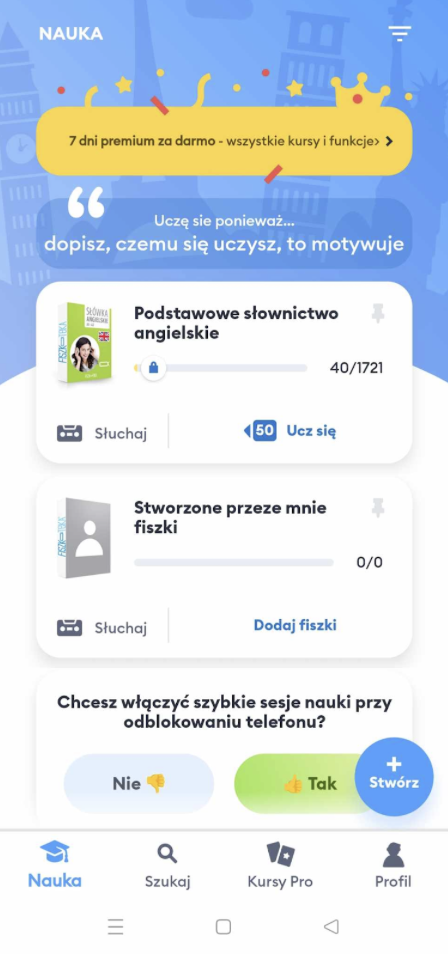
\includegraphics[width=0.3\textwidth]{chapters/chapter_3/fiszoteka.png}
    \caption{Aplikacja mobilna Fiszoteka.}
    \label{img:fiszoteka}
\end{figure}

Zalety:
\begin{itemize}[label=-]
    \item Dostępne talie językowe o różnych poziomach trudności
    \item Odczytanie przez lektora treści fiszki po zobaczeniu odpowiedzi
    \item Tryb słuchania, tytuł i treść fiszek są odczytywane po kolei przez lektora
    \item Dostęp do publicznych talii
    \item Można pobrać dokument PDF lub Mp3 z fiszek
\end{itemize}

Wady:
\begin{itemize}[label=-]
    \item Pełny dostęp do wszystkich funkcjonalności tylko za opłatą
    \item Dla bezpłatnej wersji ograniczenie liczby utworzonych fiszek do 300
    \item Reklamy w aplikacji
    \item Lektor w bezpłatnej wersji ograniczony do 20 dźwięków dziennie
    \item Brak trybu sterowania talii głosem
    \item Aplikacja ukierunkowana na uczenie się słówek
\end{itemize}

\subsection{Gizmo}

Aplikacja wykorzystuje narzędzia sztucznej inteligencji, które pozwalają na tworzenie zestawów fiszek na podstawie plików PDF, CSV lub filmów na platformie YouTube. Gizmo posiada zarówno stronę internetową, jak i aplikację mobilną na Androida i iOS.

\begin{figure}[H]
    \centering
    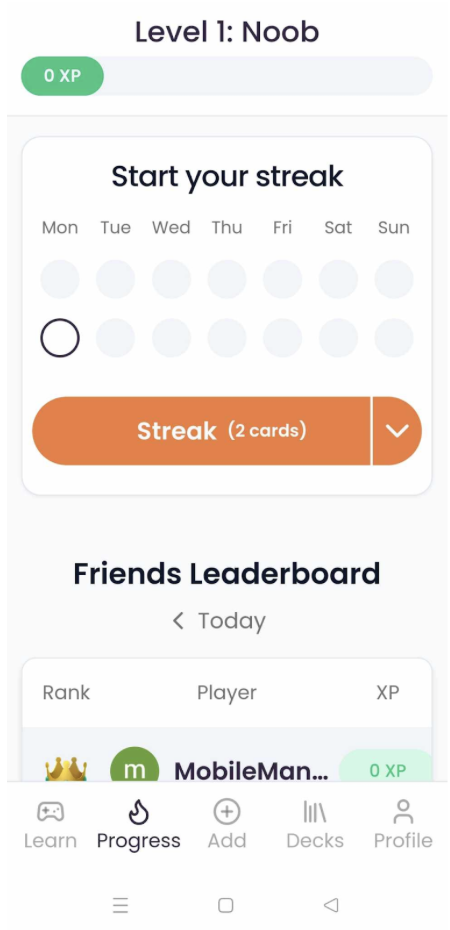
\includegraphics[width=0.3\textwidth]{chapters/chapter_3/gizmo.png}
    \caption{Aplikacja mobilna Gizmo.}
    \label{img:gizmo}
\end{figure}

Zalety:
\begin{itemize}[label=-]
    \item Brak reklam, brak opłat
    \item Zaawansowane zastosowanie AI do tworzenia fiszek
    \item Automatyczne tłumaczenie skanu na język angielski
    \item Szybki i prosty import fiszek z różnych źródeł
    \item Kalendarz passy (streak) zachęcający do nauki
    \item Przejrzysty interfejs
    \item Dostęp do publicznych talii
\end{itemize}

Wady:
\begin{itemize}[label=-]
    \item Nieumiejętne użycie AI przy tworzeniu, prowadzi do utworzenia bezsensownych talii
    \item Dużo niezagospodarowanej przestrzeni na ekranie w trybie uczenia
    \item Brak rankingu popularności talii użytkowników
    \item Domyślnie irytująca częstotliwość powiadomień
    \item Brak trybu sterowania talii głosem
\end{itemize}

\subsection{Flashcards}

Aplikacja dostępna tylko w wersji mobilnej. Ukierunkowana na uczenie się ze słuchu i tworzenie talii z użyciem mowy. Nieintuicyjny interfejs sprawia, że aplikacja jest nieprzyjazna dla nowych użytkowników.

\begin{figure}[H]
    \centering
    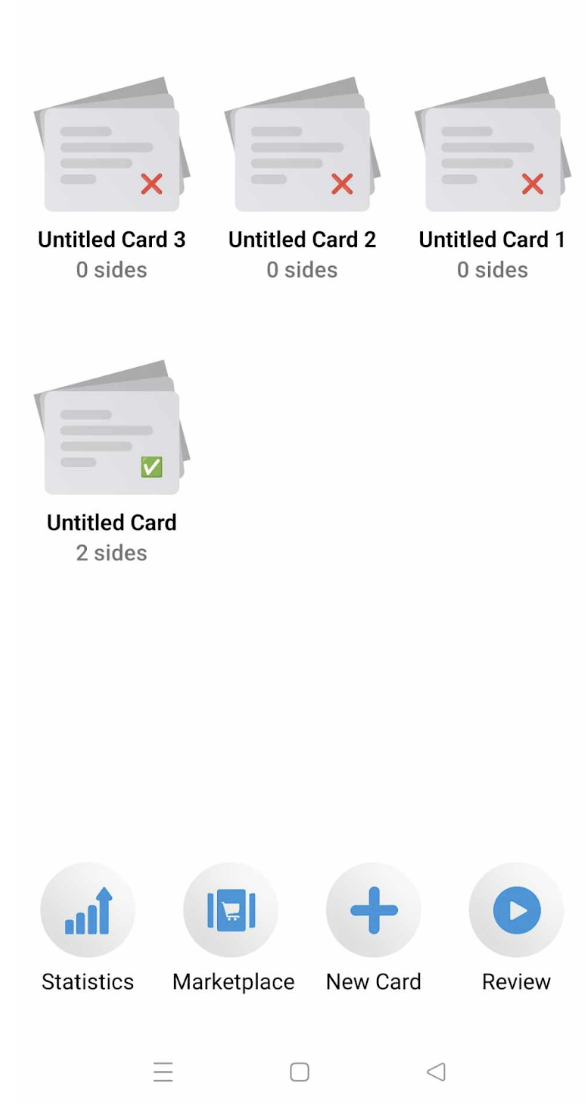
\includegraphics[width=0.3\textwidth]{chapters/chapter_3/flashcards.png}
    \caption{Aplikacja mobilna Flashcards.}
    \label{img:flashcards}
\end{figure}

Zalety:
\begin{itemize}[label=-]
    \item W trybie uczenia pozwala na korzystanie bez dotykania
    \item Możliwość tworzenia fiszek poprzez dyktowanie
    \item Brak reklam, brak opłat
\end{itemize}

Wady:
\begin{itemize}[label=-]
    \item Bardzo archaiczny interfejs
    \item Nieintuicyjny interfejs
    \item Skromna instrukcja korzystania
    \item W trybie uczenia można tylko słuchać i czekać na timer, nie ma nasłuchiwania haseł/komend
    \item Brak publicznych talii
\end{itemize}

\section{Analiza szans oraz zalet względem konkurencyjnych rozwiązań}

Podrozdział zawiera spis najważniejszych funkcjonalności, które odróżniają aplikację fiszki od innych produktów dostępnych na rynku.

\subsection{Szanse/Zalety względem konkurencyjnych rozwiązań}

Zalety:
\begin{itemize}[label=-]
    \item Sterowanie głosowe talii
    \item Generowanie treści fiszki, wykorzystując ChatGPT
    \item Ranking najpopularniejszych talii
\end{itemize}

\subsection{Wady względem konkurencyjnych rozwiązań}

Wady:
\begin{itemize}[label=-]
    \item Aplikacja dostępna tylko w języku angielskim uniemożliwia uczenie się języków obcych
    \item Brak narzędzi generowania zestawów talii z różnych formatów plików takich jak: CSV, mp4, PDF
    \item Brak możliwości generowania testów wielokrotnego wyboru lub prawda/fałsz
    \item Nie można eksportować talii do innych formatów plików takich jak PDF lub CSV
\end{itemize}

\section{Analiza ryzyka}

Podrozdział przedstawia analizę ryzyka, która ma na celu określenie i zrozumienie potencjalnych zagrożeń, które mogą wpłynąć na proces tworzenia projektu.


\newpage

\begin{longtable}{|p{2.3cm}|p{2.3cm}|p{2.3cm}|p{2.3cm}|p{2.3cm}|p{2.3cm}|}
    \hline
\textbf{Zidentyfiko- wane ryzyko [20]} & \textbf{Symptomy} & \textbf{Środki / Działania zapobiegawcze i szacowany poziom trudności ich wdrożenia} & \textbf{Środki / Działania minimalizujące wpływ na projekt – już po jego wystąpieniu i szacowany poziom trudności ich wdrożenia (1-10)} & \textbf{Ranga ryzyka (im niższa, tym mniejszy negatywny wpływ na projekt)} & \textbf{Prawdopodo- bieństwo wystąpienia (1-100\%)} \\
\hline
Błędy w kodzie [O] & Błędy w kompilacji, wyniki testów nie pokrywają się z oczekiwanym rezultatem  & Szybka identyfikacja błędów, wykonywanie testów oprogramowania & Poprawa kodu, testowanie na bieżąco nowo implementowanych funkcjonalności (4) & 10 & 80\% \\
\hline
Awaria sprzętu deweloperskiego [S] & Sprzęt przestaje działać, brak możliwości odzyskania danych & Częste commity na repozytorium & Działanie na ostatniej wersji z repozytorium (1) & 7 & 10\% \\
\hline
Niedobór umiejętności w zespole [L] & Problemy jednostek w poszczególnych zadaniach & Uzupełnianie wiedzy & Pomoc innych członków zespołu (2) & 7 & 70\% \\
\hline
Niezgodność czasowa zespołu [C]  & Osoba blokuje postęp nad projektem poprzez odpowiedzialność nad kluczowym elementem & Wcześniejsze zaplanowanie pracy & Wspólna praca nad kluczowym elementem zajęcie się zadaniami niepowiązanymi (5) & 6 & 80\% \\
\hline
Wybór nieodpowiedniej technologii [T] & Planowane rozwiązania nie są osiągalne przez wykorzystywane technologie & Dogłębna analiza potrzebnych technologii i ich możliwości/ograniczeń & Dopasowanie alternatywnych możliwych rozwiązań (8) & 5 & 50\% \\
\hline
Niedoszacowa- nie budżetu potrzebnego do utrzymania infrastruktury [B] & Budżet zbliża się do wyczerpania przed zaplanowanym terminem  & Analiza cenników wykorzystywanych produktów & Próba pozyskania inwestorów (10) & 10 & 80\% \\
\hline
ChatGPT 3.5 generuje bezsensowną treść dotycząca zagadnienia o którą został zapytany przez użytkownika [F] & Generowane treści nie nawiązują do zagadnienia, o które chat został zapytany & Próba sprecyzowania zapytania, które zostało przesłane do chatu w celu wygenerowania konkretniejszej treści & Użytkownik może zaakceptować lub odrzucić wygenerowaną treść. (4) & 7 & 50\% \\
\hline
    Przeglądarka niepoprawnie wczytuje stronę internetową [Ś] & Style strony nie wyglądają tak samo jak na stronie uruchomionej lokalnie lub na innych przeglądarkach. Pozycje elementów na stronie są inaczej rozmieszczone. & Próba dostosowania styli lub funkcjonalności do konkretnej przeglądarki.  & Uruchomienie strony internetowej na innej przeglądarce (3).   & 10 & 70\% \\
    \hline
\end{longtable}



    \chapter{Projekt w kontekście problemu}

\section{Omówienie zakresu projektu}

W odpowiedzi na zdefiniowany i omówiony w Rozdziale II problem, niniejszy projekt zakłada wytworzenie aplikacji edukacyjnej, która umożliwi naukę metodą wykorzystującą fiszki. Projekt obejmuje dostarczenie aplikacji webowej dostępnej z poziomu przeglądarki internetowej oraz aplikacji mobilnej dla urządzeń z systemem Android lub iOS. W zakres prac wlicza się także zbudowanie pełnej infrastruktury wspierającej aplikację - backend oraz serwer utrzymujący cały system.

\section{Proponowane rozwiązanie}

Projekt bazuje na kilku kluczowych założeniach, które mają na celu bezpośrednie rozwiązanie problemów opisanych w Rozdziale II:

\begin{itemize}
    \item obsługa głosowa: integracja obsługi głosowej aplikacji ma ułatwić korzystanie z niej w sytuacjach, w których użytkownik ma ograniczone możliwości fizycznej obsługi urządzenia. Dzięki temu nauka jest możliwa w każdych warunkach, co odpowiada na problem ograniczonej dostępności tradycyjnych metod nauki;
    \item narzędzie AI do tworzenia fiszek: udostępnienie narzędzia umożliwiającego automatyczne generowanie i dobieranie definicji/odpowiedzi do zagadnień w fiszkach. Pozwala przyśpieszyć i uprzystępnić proces redagowania fiszek.
\end{itemize}

\section{Grupa docelowa}

Główną grupę użytkowników stanowią uczniowie i studenci, a także osoby, które nie mają czasu na tradycyjną formę przyswajania wiedzy, na przykład czytanie lub naukę przy biurku w domowym zaciszu. Generowanie definicji przy użyciu programu ChatGPT pozwala na szybkie tworzenie zestawów fiszek, co może być bardzo wygodne dla osób ceniących sobie czas. Głosowa obsługa talii fiszek pozwala na wykonywanie sesji nauki w warunkach niesprzyjających innym formom uczenia się. Użytkownik ma możliwość powtórzenia materiału, wykonując inne obowiązki, takie jak gotowanie, sprzątanie lub inne czynności, którym nie trzeba poświęcać większej uwagi.

\section{Analiza rozwiązań konkurencji}

Ważnym aspektem tworzenia nowego produktu lub usługi jest analiza konkurencji. Dostrzeżenie wad i zalet konkurencyjnych rozwiązań pozwala na ulepszenie produktów dostępnych na rynku i dotarcie do nowej grupy klientów.

\subsection{Quizlet}

%\putimage{Aplikacja mobilna Quizlet.}{chapters/chapter_3/quizlet.png}{img:quizlet}{0.5\textwidth}

Jedna z pierwszych dostępnych na rynku aplikacja do fiszek. Utworzone w 2005 roku narzędzie do nauki zgromadziło ogromną bazę użytkowników szacowaną na około 50 milionów. Quizlet posiada stronę internetową i aplikacje mobilną dostępne na Android i IOS.

\begin{figure}[H]
    \centering
    
\includegraphics[width=0.3\textwidth]{chapters/chapter_3/quizlet.png}
    \caption{Aplikacja mobilna Quizlet.}
    \label{img:quizlet}
\end{figure}

Zalety:
\begin{itemize}[label=-]
    \item Możliwość tworzenia testów w różnych trybach: prawda/fałsz, wielokrotny wybór, pisemny
    \item Odczytanie przez lektora treści fiszki poprzez kliknięcie przycisku
    \item Dostęp do materiałów, które zostały zweryfikowane przez ekspertów
    \item Personalizacja fiszek za pomocą obrazów i dźwięków
    \item Pozwala na wyszukiwanie talii innych użytkowników
\end{itemize}

Wady:
\begin{itemize}[label=-]
    \item Reklamy w aplikacji
    \item Pełny dostęp do wszystkich funkcjonalności tylko za opłatą
    \item Brak rankingu popularności talii użytkowników, co pozwalałoby na łatwy dostęp do innych talii
    \item Brak trybu sterowania talii głosem
\end{itemize}

\subsection{Fiszkoteka}

Polski portal do nauki metodą fiszek ukierunkowany na naukę języków obcych. Oprócz strony internetowej aplikacja dostępna na system Android lub iOS.

\begin{figure}[H]
    \centering
    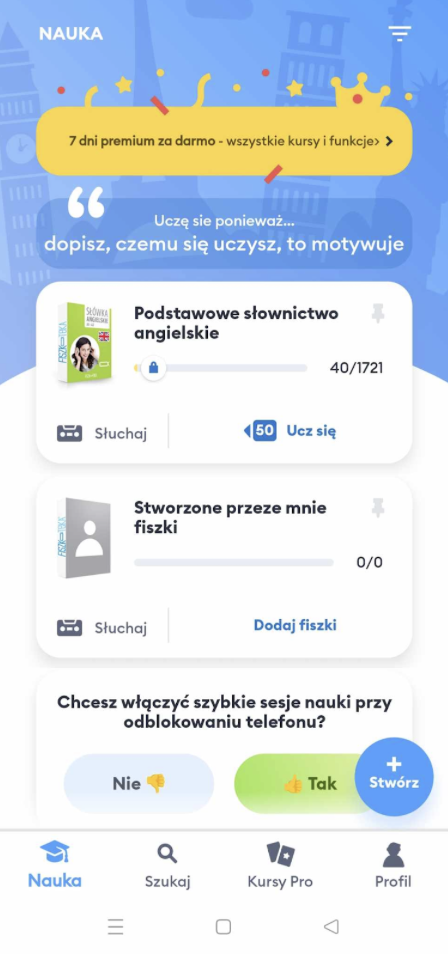
\includegraphics[width=0.3\textwidth]{chapters/chapter_3/fiszoteka.png}
    \caption{Aplikacja mobilna Fiszoteka.}
    \label{img:fiszoteka}
\end{figure}

Zalety:
\begin{itemize}[label=-]
    \item Dostępne talie językowe o różnych poziomach trudności
    \item Odczytanie przez lektora treści fiszki po zobaczeniu odpowiedzi
    \item Tryb słuchania, tytuł i treść fiszek są odczytywane po kolei przez lektora
    \item Dostęp do publicznych talii
    \item Można pobrać dokument PDF lub Mp3 z fiszek
\end{itemize}

Wady:
\begin{itemize}[label=-]
    \item Pełny dostęp do wszystkich funkcjonalności tylko za opłatą
    \item Dla bezpłatnej wersji ograniczenie liczby utworzonych fiszek do 300
    \item Reklamy w aplikacji
    \item Lektor w bezpłatnej wersji ograniczony do 20 dźwięków dziennie
    \item Brak trybu sterowania talii głosem
    \item Aplikacja ukierunkowana na uczenie się słówek
\end{itemize}

\subsection{Gizmo}

Aplikacja wykorzystuje narzędzia sztucznej inteligencji, które pozwalają na tworzenie zestawów fiszek na podstawie plików PDF, CSV lub filmów na platformie YouTube. Gizmo posiada zarówno stronę internetową, jak i aplikację mobilną na Androida i iOS.

\begin{figure}[H]
    \centering
    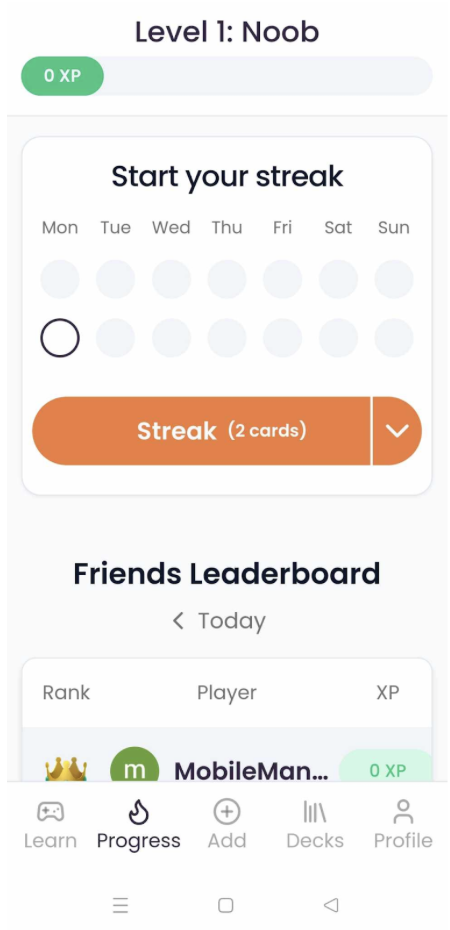
\includegraphics[width=0.3\textwidth]{chapters/chapter_3/gizmo.png}
    \caption{Aplikacja mobilna Gizmo.}
    \label{img:gizmo}
\end{figure}

Zalety:
\begin{itemize}[label=-]
    \item Brak reklam, brak opłat
    \item Zaawansowane zastosowanie AI do tworzenia fiszek
    \item Automatyczne tłumaczenie skanu na język angielski
    \item Szybki i prosty import fiszek z różnych źródeł
    \item Kalendarz passy (streak) zachęcający do nauki
    \item Przejrzysty interfejs
    \item Dostęp do publicznych talii
\end{itemize}

Wady:
\begin{itemize}[label=-]
    \item Nieumiejętne użycie AI przy tworzeniu, prowadzi do utworzenia bezsensownych talii
    \item Dużo niezagospodarowanej przestrzeni na ekranie w trybie uczenia
    \item Brak rankingu popularności talii użytkowników
    \item Domyślnie irytująca częstotliwość powiadomień
    \item Brak trybu sterowania talii głosem
\end{itemize}

\subsection{Flashcards}

Aplikacja dostępna tylko w wersji mobilnej. Ukierunkowana na uczenie się ze słuchu i tworzenie talii z użyciem mowy. Nieintuicyjny interfejs sprawia, że aplikacja jest nieprzyjazna dla nowych użytkowników.

\begin{figure}[H]
    \centering
    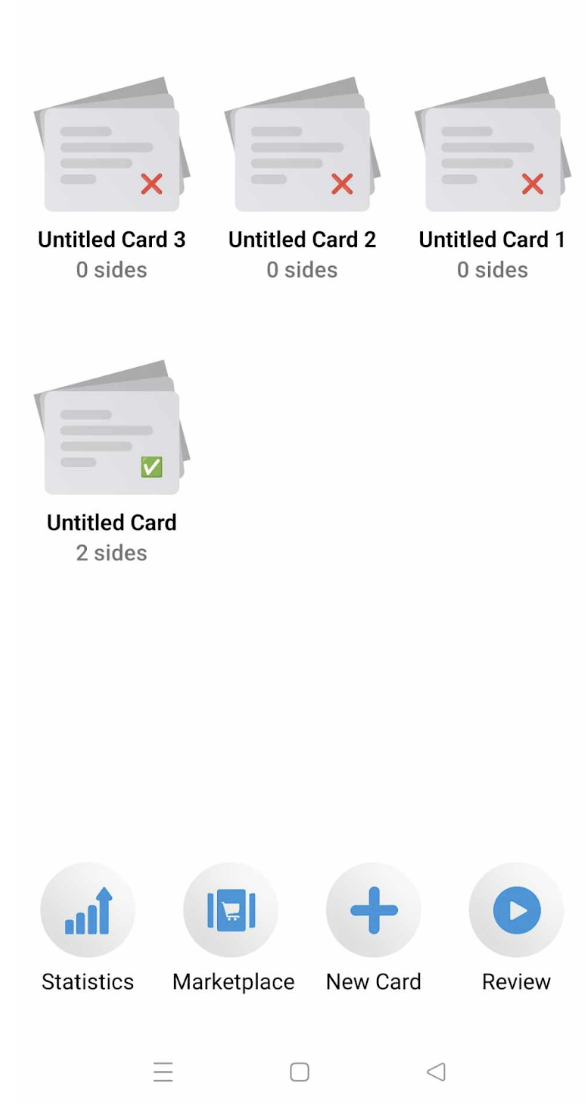
\includegraphics[width=0.3\textwidth]{chapters/chapter_3/flashcards.png}
    \caption{Aplikacja mobilna Flashcards.}
    \label{img:flashcards}
\end{figure}

Zalety:
\begin{itemize}[label=-]
    \item W trybie uczenia pozwala na korzystanie bez dotykania
    \item Możliwość tworzenia fiszek poprzez dyktowanie
    \item Brak reklam, brak opłat
\end{itemize}

Wady:
\begin{itemize}[label=-]
    \item Bardzo archaiczny interfejs
    \item Nieintuicyjny interfejs
    \item Skromna instrukcja korzystania
    \item W trybie uczenia można tylko słuchać i czekać na timer, nie ma nasłuchiwania haseł/komend
    \item Brak publicznych talii
\end{itemize}

\section{Analiza szans oraz zalet względem konkurencyjnych rozwiązań}

Podrozdział zawiera spis najważniejszych funkcjonalności, które odróżniają aplikację fiszki od innych produktów dostępnych na rynku.

\subsection{Szanse/Zalety względem konkurencyjnych rozwiązań}

Zalety:
\begin{itemize}[label=-]
    \item Sterowanie głosowe talii
    \item Generowanie treści fiszki, wykorzystując ChatGPT
    \item Ranking najpopularniejszych talii
\end{itemize}

\subsection{Wady względem konkurencyjnych rozwiązań}

Wady:
\begin{itemize}[label=-]
    \item Aplikacja dostępna tylko w języku angielskim uniemożliwia uczenie się języków obcych
    \item Brak narzędzi generowania zestawów talii z różnych formatów plików takich jak: CSV, mp4, PDF
    \item Brak możliwości generowania testów wielokrotnego wyboru lub prawda/fałsz
    \item Nie można eksportować talii do innych formatów plików takich jak PDF lub CSV
\end{itemize}

\section{Analiza ryzyka}

Podrozdział przedstawia analizę ryzyka, która ma na celu określenie i zrozumienie potencjalnych zagrożeń, które mogą wpłynąć na proces tworzenia projektu.


\newpage

\begin{longtable}{|p{2.3cm}|p{2.3cm}|p{2.3cm}|p{2.3cm}|p{2.3cm}|p{2.3cm}|}
    \hline
\textbf{Zidentyfiko- wane ryzyko [20]} & \textbf{Symptomy} & \textbf{Środki / Działania zapobiegawcze i szacowany poziom trudności ich wdrożenia} & \textbf{Środki / Działania minimalizujące wpływ na projekt – już po jego wystąpieniu i szacowany poziom trudności ich wdrożenia (1-10)} & \textbf{Ranga ryzyka (im niższa, tym mniejszy negatywny wpływ na projekt)} & \textbf{Prawdopodo- bieństwo wystąpienia (1-100\%)} \\
\hline
Błędy w kodzie [O] & Błędy w kompilacji, wyniki testów nie pokrywają się z oczekiwanym rezultatem  & Szybka identyfikacja błędów, wykonywanie testów oprogramowania & Poprawa kodu, testowanie na bieżąco nowo implementowanych funkcjonalności (4) & 10 & 80\% \\
\hline
Awaria sprzętu deweloperskiego [S] & Sprzęt przestaje działać, brak możliwości odzyskania danych & Częste commity na repozytorium & Działanie na ostatniej wersji z repozytorium (1) & 7 & 10\% \\
\hline
Niedobór umiejętności w zespole [L] & Problemy jednostek w poszczególnych zadaniach & Uzupełnianie wiedzy & Pomoc innych członków zespołu (2) & 7 & 70\% \\
\hline
Niezgodność czasowa zespołu [C]  & Osoba blokuje postęp nad projektem poprzez odpowiedzialność nad kluczowym elementem & Wcześniejsze zaplanowanie pracy & Wspólna praca nad kluczowym elementem zajęcie się zadaniami niepowiązanymi (5) & 6 & 80\% \\
\hline
Wybór nieodpowiedniej technologii [T] & Planowane rozwiązania nie są osiągalne przez wykorzystywane technologie & Dogłębna analiza potrzebnych technologii i ich możliwości/ograniczeń & Dopasowanie alternatywnych możliwych rozwiązań (8) & 5 & 50\% \\
\hline
Niedoszacowa- nie budżetu potrzebnego do utrzymania infrastruktury [B] & Budżet zbliża się do wyczerpania przed zaplanowanym terminem  & Analiza cenników wykorzystywanych produktów & Próba pozyskania inwestorów (10) & 10 & 80\% \\
\hline
ChatGPT 3.5 generuje bezsensowną treść dotycząca zagadnienia o którą został zapytany przez użytkownika [F] & Generowane treści nie nawiązują do zagadnienia, o które chat został zapytany & Próba sprecyzowania zapytania, które zostało przesłane do chatu w celu wygenerowania konkretniejszej treści & Użytkownik może zaakceptować lub odrzucić wygenerowaną treść. (4) & 7 & 50\% \\
\hline
    Przeglądarka niepoprawnie wczytuje stronę internetową [Ś] & Style strony nie wyglądają tak samo jak na stronie uruchomionej lokalnie lub na innych przeglądarkach. Pozycje elementów na stronie są inaczej rozmieszczone. & Próba dostosowania styli lub funkcjonalności do konkretnej przeglądarki.  & Uruchomienie strony internetowej na innej przeglądarce (3).   & 10 & 70\% \\
    \hline
\end{longtable}



    \chapter{Projekt w kontekście problemu}

\section{Omówienie zakresu projektu}

W odpowiedzi na zdefiniowany i omówiony w Rozdziale II problem, niniejszy projekt zakłada wytworzenie aplikacji edukacyjnej, która umożliwi naukę metodą wykorzystującą fiszki. Projekt obejmuje dostarczenie aplikacji webowej dostępnej z poziomu przeglądarki internetowej oraz aplikacji mobilnej dla urządzeń z systemem Android lub iOS. W zakres prac wlicza się także zbudowanie pełnej infrastruktury wspierającej aplikację - backend oraz serwer utrzymujący cały system.

\section{Proponowane rozwiązanie}

Projekt bazuje na kilku kluczowych założeniach, które mają na celu bezpośrednie rozwiązanie problemów opisanych w Rozdziale II:

\begin{itemize}
    \item obsługa głosowa: integracja obsługi głosowej aplikacji ma ułatwić korzystanie z niej w sytuacjach, w których użytkownik ma ograniczone możliwości fizycznej obsługi urządzenia. Dzięki temu nauka jest możliwa w każdych warunkach, co odpowiada na problem ograniczonej dostępności tradycyjnych metod nauki;
    \item narzędzie AI do tworzenia fiszek: udostępnienie narzędzia umożliwiającego automatyczne generowanie i dobieranie definicji/odpowiedzi do zagadnień w fiszkach. Pozwala przyśpieszyć i uprzystępnić proces redagowania fiszek.
\end{itemize}

\section{Grupa docelowa}

Główną grupę użytkowników stanowią uczniowie i studenci, a także osoby, które nie mają czasu na tradycyjną formę przyswajania wiedzy, na przykład czytanie lub naukę przy biurku w domowym zaciszu. Generowanie definicji przy użyciu programu ChatGPT pozwala na szybkie tworzenie zestawów fiszek, co może być bardzo wygodne dla osób ceniących sobie czas. Głosowa obsługa talii fiszek pozwala na wykonywanie sesji nauki w warunkach niesprzyjających innym formom uczenia się. Użytkownik ma możliwość powtórzenia materiału, wykonując inne obowiązki, takie jak gotowanie, sprzątanie lub inne czynności, którym nie trzeba poświęcać większej uwagi.

\section{Analiza rozwiązań konkurencji}

Ważnym aspektem tworzenia nowego produktu lub usługi jest analiza konkurencji. Dostrzeżenie wad i zalet konkurencyjnych rozwiązań pozwala na ulepszenie produktów dostępnych na rynku i dotarcie do nowej grupy klientów.

\subsection{Quizlet}

%\putimage{Aplikacja mobilna Quizlet.}{chapters/chapter_3/quizlet.png}{img:quizlet}{0.5\textwidth}

Jedna z pierwszych dostępnych na rynku aplikacja do fiszek. Utworzone w 2005 roku narzędzie do nauki zgromadziło ogromną bazę użytkowników szacowaną na około 50 milionów. Quizlet posiada stronę internetową i aplikacje mobilną dostępne na Android i IOS.

\begin{figure}[H]
    \centering
    
\includegraphics[width=0.3\textwidth]{chapters/chapter_3/quizlet.png}
    \caption{Aplikacja mobilna Quizlet.}
    \label{img:quizlet}
\end{figure}

Zalety:
\begin{itemize}[label=-]
    \item Możliwość tworzenia testów w różnych trybach: prawda/fałsz, wielokrotny wybór, pisemny
    \item Odczytanie przez lektora treści fiszki poprzez kliknięcie przycisku
    \item Dostęp do materiałów, które zostały zweryfikowane przez ekspertów
    \item Personalizacja fiszek za pomocą obrazów i dźwięków
    \item Pozwala na wyszukiwanie talii innych użytkowników
\end{itemize}

Wady:
\begin{itemize}[label=-]
    \item Reklamy w aplikacji
    \item Pełny dostęp do wszystkich funkcjonalności tylko za opłatą
    \item Brak rankingu popularności talii użytkowników, co pozwalałoby na łatwy dostęp do innych talii
    \item Brak trybu sterowania talii głosem
\end{itemize}

\subsection{Fiszkoteka}

Polski portal do nauki metodą fiszek ukierunkowany na naukę języków obcych. Oprócz strony internetowej aplikacja dostępna na system Android lub iOS.

\begin{figure}[H]
    \centering
    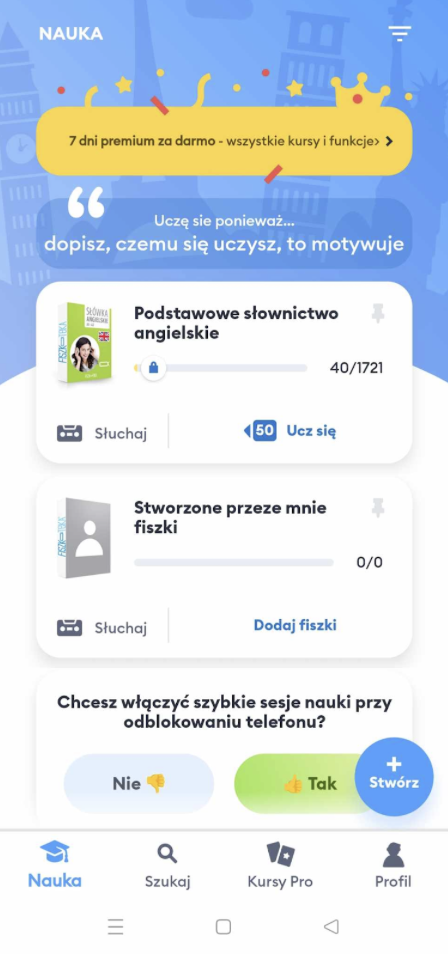
\includegraphics[width=0.3\textwidth]{chapters/chapter_3/fiszoteka.png}
    \caption{Aplikacja mobilna Fiszoteka.}
    \label{img:fiszoteka}
\end{figure}

Zalety:
\begin{itemize}[label=-]
    \item Dostępne talie językowe o różnych poziomach trudności
    \item Odczytanie przez lektora treści fiszki po zobaczeniu odpowiedzi
    \item Tryb słuchania, tytuł i treść fiszek są odczytywane po kolei przez lektora
    \item Dostęp do publicznych talii
    \item Można pobrać dokument PDF lub Mp3 z fiszek
\end{itemize}

Wady:
\begin{itemize}[label=-]
    \item Pełny dostęp do wszystkich funkcjonalności tylko za opłatą
    \item Dla bezpłatnej wersji ograniczenie liczby utworzonych fiszek do 300
    \item Reklamy w aplikacji
    \item Lektor w bezpłatnej wersji ograniczony do 20 dźwięków dziennie
    \item Brak trybu sterowania talii głosem
    \item Aplikacja ukierunkowana na uczenie się słówek
\end{itemize}

\subsection{Gizmo}

Aplikacja wykorzystuje narzędzia sztucznej inteligencji, które pozwalają na tworzenie zestawów fiszek na podstawie plików PDF, CSV lub filmów na platformie YouTube. Gizmo posiada zarówno stronę internetową, jak i aplikację mobilną na Androida i iOS.

\begin{figure}[H]
    \centering
    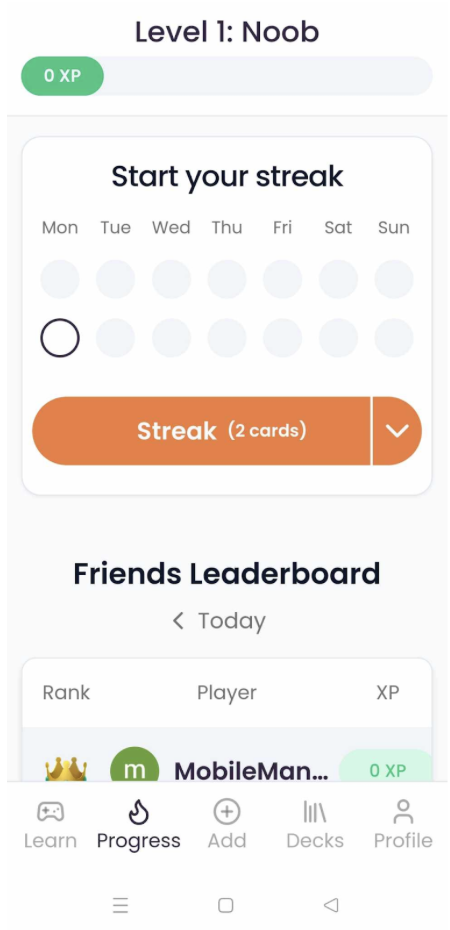
\includegraphics[width=0.3\textwidth]{chapters/chapter_3/gizmo.png}
    \caption{Aplikacja mobilna Gizmo.}
    \label{img:gizmo}
\end{figure}

Zalety:
\begin{itemize}[label=-]
    \item Brak reklam, brak opłat
    \item Zaawansowane zastosowanie AI do tworzenia fiszek
    \item Automatyczne tłumaczenie skanu na język angielski
    \item Szybki i prosty import fiszek z różnych źródeł
    \item Kalendarz passy (streak) zachęcający do nauki
    \item Przejrzysty interfejs
    \item Dostęp do publicznych talii
\end{itemize}

Wady:
\begin{itemize}[label=-]
    \item Nieumiejętne użycie AI przy tworzeniu, prowadzi do utworzenia bezsensownych talii
    \item Dużo niezagospodarowanej przestrzeni na ekranie w trybie uczenia
    \item Brak rankingu popularności talii użytkowników
    \item Domyślnie irytująca częstotliwość powiadomień
    \item Brak trybu sterowania talii głosem
\end{itemize}

\subsection{Flashcards}

Aplikacja dostępna tylko w wersji mobilnej. Ukierunkowana na uczenie się ze słuchu i tworzenie talii z użyciem mowy. Nieintuicyjny interfejs sprawia, że aplikacja jest nieprzyjazna dla nowych użytkowników.

\begin{figure}[H]
    \centering
    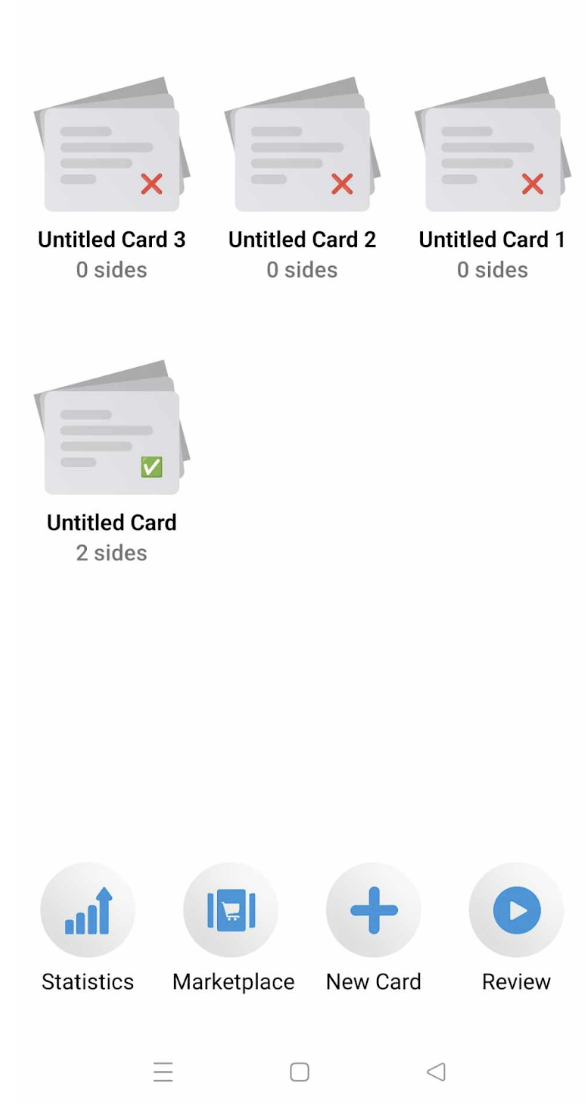
\includegraphics[width=0.3\textwidth]{chapters/chapter_3/flashcards.png}
    \caption{Aplikacja mobilna Flashcards.}
    \label{img:flashcards}
\end{figure}

Zalety:
\begin{itemize}[label=-]
    \item W trybie uczenia pozwala na korzystanie bez dotykania
    \item Możliwość tworzenia fiszek poprzez dyktowanie
    \item Brak reklam, brak opłat
\end{itemize}

Wady:
\begin{itemize}[label=-]
    \item Bardzo archaiczny interfejs
    \item Nieintuicyjny interfejs
    \item Skromna instrukcja korzystania
    \item W trybie uczenia można tylko słuchać i czekać na timer, nie ma nasłuchiwania haseł/komend
    \item Brak publicznych talii
\end{itemize}

\section{Analiza szans oraz zalet względem konkurencyjnych rozwiązań}

Podrozdział zawiera spis najważniejszych funkcjonalności, które odróżniają aplikację fiszki od innych produktów dostępnych na rynku.

\subsection{Szanse/Zalety względem konkurencyjnych rozwiązań}

Zalety:
\begin{itemize}[label=-]
    \item Sterowanie głosowe talii
    \item Generowanie treści fiszki, wykorzystując ChatGPT
    \item Ranking najpopularniejszych talii
\end{itemize}

\subsection{Wady względem konkurencyjnych rozwiązań}

Wady:
\begin{itemize}[label=-]
    \item Aplikacja dostępna tylko w języku angielskim uniemożliwia uczenie się języków obcych
    \item Brak narzędzi generowania zestawów talii z różnych formatów plików takich jak: CSV, mp4, PDF
    \item Brak możliwości generowania testów wielokrotnego wyboru lub prawda/fałsz
    \item Nie można eksportować talii do innych formatów plików takich jak PDF lub CSV
\end{itemize}

\section{Analiza ryzyka}

Podrozdział przedstawia analizę ryzyka, która ma na celu określenie i zrozumienie potencjalnych zagrożeń, które mogą wpłynąć na proces tworzenia projektu.


\newpage

\begin{longtable}{|p{2.3cm}|p{2.3cm}|p{2.3cm}|p{2.3cm}|p{2.3cm}|p{2.3cm}|}
    \hline
\textbf{Zidentyfiko- wane ryzyko [20]} & \textbf{Symptomy} & \textbf{Środki / Działania zapobiegawcze i szacowany poziom trudności ich wdrożenia} & \textbf{Środki / Działania minimalizujące wpływ na projekt – już po jego wystąpieniu i szacowany poziom trudności ich wdrożenia (1-10)} & \textbf{Ranga ryzyka (im niższa, tym mniejszy negatywny wpływ na projekt)} & \textbf{Prawdopodo- bieństwo wystąpienia (1-100\%)} \\
\hline
Błędy w kodzie [O] & Błędy w kompilacji, wyniki testów nie pokrywają się z oczekiwanym rezultatem  & Szybka identyfikacja błędów, wykonywanie testów oprogramowania & Poprawa kodu, testowanie na bieżąco nowo implementowanych funkcjonalności (4) & 10 & 80\% \\
\hline
Awaria sprzętu deweloperskiego [S] & Sprzęt przestaje działać, brak możliwości odzyskania danych & Częste commity na repozytorium & Działanie na ostatniej wersji z repozytorium (1) & 7 & 10\% \\
\hline
Niedobór umiejętności w zespole [L] & Problemy jednostek w poszczególnych zadaniach & Uzupełnianie wiedzy & Pomoc innych członków zespołu (2) & 7 & 70\% \\
\hline
Niezgodność czasowa zespołu [C]  & Osoba blokuje postęp nad projektem poprzez odpowiedzialność nad kluczowym elementem & Wcześniejsze zaplanowanie pracy & Wspólna praca nad kluczowym elementem zajęcie się zadaniami niepowiązanymi (5) & 6 & 80\% \\
\hline
Wybór nieodpowiedniej technologii [T] & Planowane rozwiązania nie są osiągalne przez wykorzystywane technologie & Dogłębna analiza potrzebnych technologii i ich możliwości/ograniczeń & Dopasowanie alternatywnych możliwych rozwiązań (8) & 5 & 50\% \\
\hline
Niedoszacowa- nie budżetu potrzebnego do utrzymania infrastruktury [B] & Budżet zbliża się do wyczerpania przed zaplanowanym terminem  & Analiza cenników wykorzystywanych produktów & Próba pozyskania inwestorów (10) & 10 & 80\% \\
\hline
ChatGPT 3.5 generuje bezsensowną treść dotycząca zagadnienia o którą został zapytany przez użytkownika [F] & Generowane treści nie nawiązują do zagadnienia, o które chat został zapytany & Próba sprecyzowania zapytania, które zostało przesłane do chatu w celu wygenerowania konkretniejszej treści & Użytkownik może zaakceptować lub odrzucić wygenerowaną treść. (4) & 7 & 50\% \\
\hline
    Przeglądarka niepoprawnie wczytuje stronę internetową [Ś] & Style strony nie wyglądają tak samo jak na stronie uruchomionej lokalnie lub na innych przeglądarkach. Pozycje elementów na stronie są inaczej rozmieszczone. & Próba dostosowania styli lub funkcjonalności do konkretnej przeglądarki.  & Uruchomienie strony internetowej na innej przeglądarce (3).   & 10 & 70\% \\
    \hline
\end{longtable}



  %  \chapter{Projekt w kontekście problemu}

\section{Omówienie zakresu projektu}

W odpowiedzi na zdefiniowany i omówiony w Rozdziale II problem, niniejszy projekt zakłada wytworzenie aplikacji edukacyjnej, która umożliwi naukę metodą wykorzystującą fiszki. Projekt obejmuje dostarczenie aplikacji webowej dostępnej z poziomu przeglądarki internetowej oraz aplikacji mobilnej dla urządzeń z systemem Android lub iOS. W zakres prac wlicza się także zbudowanie pełnej infrastruktury wspierającej aplikację - backend oraz serwer utrzymujący cały system.

\section{Proponowane rozwiązanie}

Projekt bazuje na kilku kluczowych założeniach, które mają na celu bezpośrednie rozwiązanie problemów opisanych w Rozdziale II:

\begin{itemize}
    \item obsługa głosowa: integracja obsługi głosowej aplikacji ma ułatwić korzystanie z niej w sytuacjach, w których użytkownik ma ograniczone możliwości fizycznej obsługi urządzenia. Dzięki temu nauka jest możliwa w każdych warunkach, co odpowiada na problem ograniczonej dostępności tradycyjnych metod nauki;
    \item narzędzie AI do tworzenia fiszek: udostępnienie narzędzia umożliwiającego automatyczne generowanie i dobieranie definicji/odpowiedzi do zagadnień w fiszkach. Pozwala przyśpieszyć i uprzystępnić proces redagowania fiszek.
\end{itemize}

\section{Grupa docelowa}

Główną grupę użytkowników stanowią uczniowie i studenci, a także osoby, które nie mają czasu na tradycyjną formę przyswajania wiedzy, na przykład czytanie lub naukę przy biurku w domowym zaciszu. Generowanie definicji przy użyciu programu ChatGPT pozwala na szybkie tworzenie zestawów fiszek, co może być bardzo wygodne dla osób ceniących sobie czas. Głosowa obsługa talii fiszek pozwala na wykonywanie sesji nauki w warunkach niesprzyjających innym formom uczenia się. Użytkownik ma możliwość powtórzenia materiału, wykonując inne obowiązki, takie jak gotowanie, sprzątanie lub inne czynności, którym nie trzeba poświęcać większej uwagi.

\section{Analiza rozwiązań konkurencji}

Ważnym aspektem tworzenia nowego produktu lub usługi jest analiza konkurencji. Dostrzeżenie wad i zalet konkurencyjnych rozwiązań pozwala na ulepszenie produktów dostępnych na rynku i dotarcie do nowej grupy klientów.

\subsection{Quizlet}

%\putimage{Aplikacja mobilna Quizlet.}{chapters/chapter_3/quizlet.png}{img:quizlet}{0.5\textwidth}

Jedna z pierwszych dostępnych na rynku aplikacja do fiszek. Utworzone w 2005 roku narzędzie do nauki zgromadziło ogromną bazę użytkowników szacowaną na około 50 milionów. Quizlet posiada stronę internetową i aplikacje mobilną dostępne na Android i IOS.

\begin{figure}[H]
    \centering
    
\includegraphics[width=0.3\textwidth]{chapters/chapter_3/quizlet.png}
    \caption{Aplikacja mobilna Quizlet.}
    \label{img:quizlet}
\end{figure}

Zalety:
\begin{itemize}[label=-]
    \item Możliwość tworzenia testów w różnych trybach: prawda/fałsz, wielokrotny wybór, pisemny
    \item Odczytanie przez lektora treści fiszki poprzez kliknięcie przycisku
    \item Dostęp do materiałów, które zostały zweryfikowane przez ekspertów
    \item Personalizacja fiszek za pomocą obrazów i dźwięków
    \item Pozwala na wyszukiwanie talii innych użytkowników
\end{itemize}

Wady:
\begin{itemize}[label=-]
    \item Reklamy w aplikacji
    \item Pełny dostęp do wszystkich funkcjonalności tylko za opłatą
    \item Brak rankingu popularności talii użytkowników, co pozwalałoby na łatwy dostęp do innych talii
    \item Brak trybu sterowania talii głosem
\end{itemize}

\subsection{Fiszkoteka}

Polski portal do nauki metodą fiszek ukierunkowany na naukę języków obcych. Oprócz strony internetowej aplikacja dostępna na system Android lub iOS.

\begin{figure}[H]
    \centering
    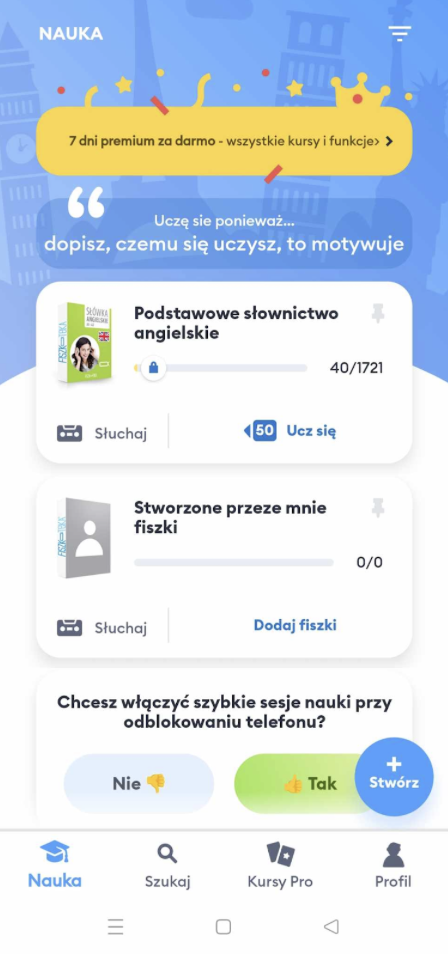
\includegraphics[width=0.3\textwidth]{chapters/chapter_3/fiszoteka.png}
    \caption{Aplikacja mobilna Fiszoteka.}
    \label{img:fiszoteka}
\end{figure}

Zalety:
\begin{itemize}[label=-]
    \item Dostępne talie językowe o różnych poziomach trudności
    \item Odczytanie przez lektora treści fiszki po zobaczeniu odpowiedzi
    \item Tryb słuchania, tytuł i treść fiszek są odczytywane po kolei przez lektora
    \item Dostęp do publicznych talii
    \item Można pobrać dokument PDF lub Mp3 z fiszek
\end{itemize}

Wady:
\begin{itemize}[label=-]
    \item Pełny dostęp do wszystkich funkcjonalności tylko za opłatą
    \item Dla bezpłatnej wersji ograniczenie liczby utworzonych fiszek do 300
    \item Reklamy w aplikacji
    \item Lektor w bezpłatnej wersji ograniczony do 20 dźwięków dziennie
    \item Brak trybu sterowania talii głosem
    \item Aplikacja ukierunkowana na uczenie się słówek
\end{itemize}

\subsection{Gizmo}

Aplikacja wykorzystuje narzędzia sztucznej inteligencji, które pozwalają na tworzenie zestawów fiszek na podstawie plików PDF, CSV lub filmów na platformie YouTube. Gizmo posiada zarówno stronę internetową, jak i aplikację mobilną na Androida i iOS.

\begin{figure}[H]
    \centering
    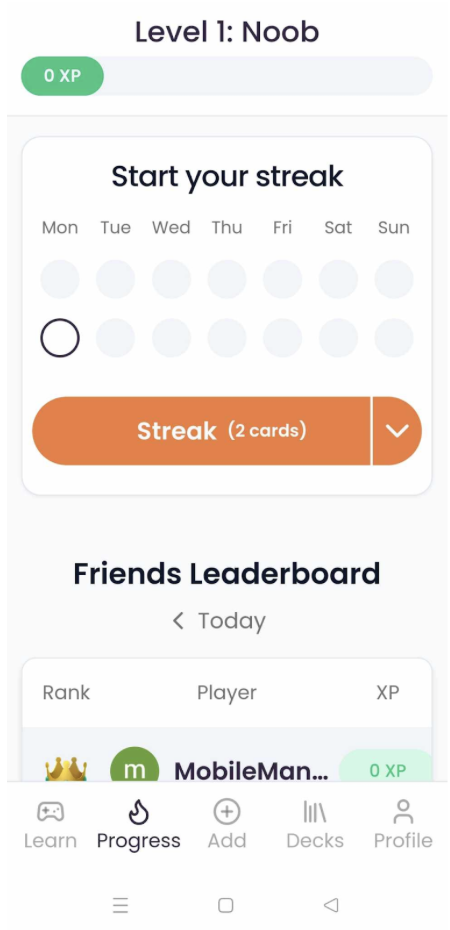
\includegraphics[width=0.3\textwidth]{chapters/chapter_3/gizmo.png}
    \caption{Aplikacja mobilna Gizmo.}
    \label{img:gizmo}
\end{figure}

Zalety:
\begin{itemize}[label=-]
    \item Brak reklam, brak opłat
    \item Zaawansowane zastosowanie AI do tworzenia fiszek
    \item Automatyczne tłumaczenie skanu na język angielski
    \item Szybki i prosty import fiszek z różnych źródeł
    \item Kalendarz passy (streak) zachęcający do nauki
    \item Przejrzysty interfejs
    \item Dostęp do publicznych talii
\end{itemize}

Wady:
\begin{itemize}[label=-]
    \item Nieumiejętne użycie AI przy tworzeniu, prowadzi do utworzenia bezsensownych talii
    \item Dużo niezagospodarowanej przestrzeni na ekranie w trybie uczenia
    \item Brak rankingu popularności talii użytkowników
    \item Domyślnie irytująca częstotliwość powiadomień
    \item Brak trybu sterowania talii głosem
\end{itemize}

\subsection{Flashcards}

Aplikacja dostępna tylko w wersji mobilnej. Ukierunkowana na uczenie się ze słuchu i tworzenie talii z użyciem mowy. Nieintuicyjny interfejs sprawia, że aplikacja jest nieprzyjazna dla nowych użytkowników.

\begin{figure}[H]
    \centering
    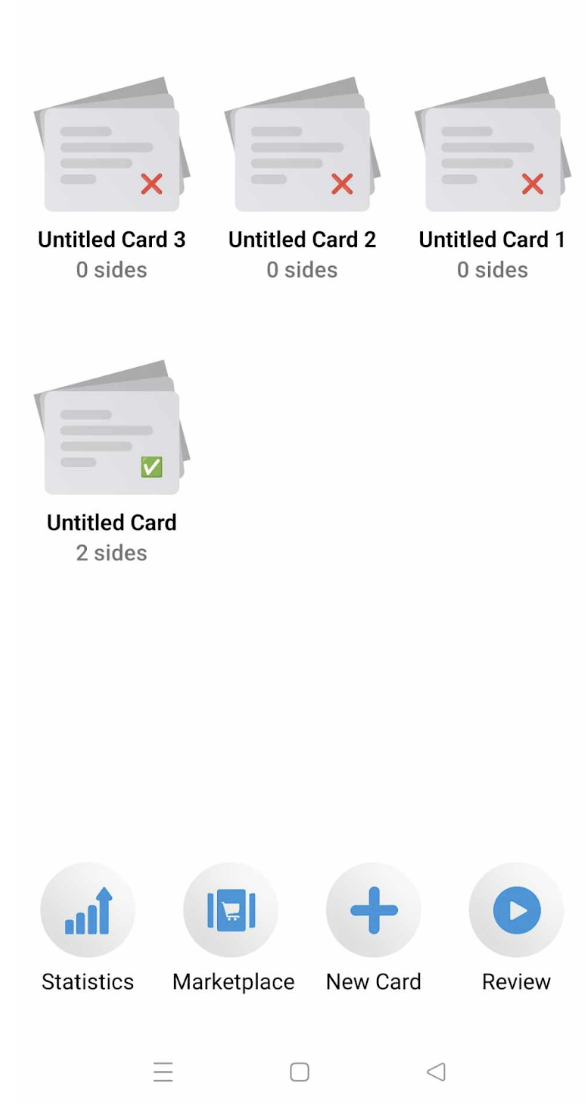
\includegraphics[width=0.3\textwidth]{chapters/chapter_3/flashcards.png}
    \caption{Aplikacja mobilna Flashcards.}
    \label{img:flashcards}
\end{figure}

Zalety:
\begin{itemize}[label=-]
    \item W trybie uczenia pozwala na korzystanie bez dotykania
    \item Możliwość tworzenia fiszek poprzez dyktowanie
    \item Brak reklam, brak opłat
\end{itemize}

Wady:
\begin{itemize}[label=-]
    \item Bardzo archaiczny interfejs
    \item Nieintuicyjny interfejs
    \item Skromna instrukcja korzystania
    \item W trybie uczenia można tylko słuchać i czekać na timer, nie ma nasłuchiwania haseł/komend
    \item Brak publicznych talii
\end{itemize}

\section{Analiza szans oraz zalet względem konkurencyjnych rozwiązań}

Podrozdział zawiera spis najważniejszych funkcjonalności, które odróżniają aplikację fiszki od innych produktów dostępnych na rynku.

\subsection{Szanse/Zalety względem konkurencyjnych rozwiązań}

Zalety:
\begin{itemize}[label=-]
    \item Sterowanie głosowe talii
    \item Generowanie treści fiszki, wykorzystując ChatGPT
    \item Ranking najpopularniejszych talii
\end{itemize}

\subsection{Wady względem konkurencyjnych rozwiązań}

Wady:
\begin{itemize}[label=-]
    \item Aplikacja dostępna tylko w języku angielskim uniemożliwia uczenie się języków obcych
    \item Brak narzędzi generowania zestawów talii z różnych formatów plików takich jak: CSV, mp4, PDF
    \item Brak możliwości generowania testów wielokrotnego wyboru lub prawda/fałsz
    \item Nie można eksportować talii do innych formatów plików takich jak PDF lub CSV
\end{itemize}

\section{Analiza ryzyka}

Podrozdział przedstawia analizę ryzyka, która ma na celu określenie i zrozumienie potencjalnych zagrożeń, które mogą wpłynąć na proces tworzenia projektu.


\newpage

\begin{longtable}{|p{2.3cm}|p{2.3cm}|p{2.3cm}|p{2.3cm}|p{2.3cm}|p{2.3cm}|}
    \hline
\textbf{Zidentyfiko- wane ryzyko [20]} & \textbf{Symptomy} & \textbf{Środki / Działania zapobiegawcze i szacowany poziom trudności ich wdrożenia} & \textbf{Środki / Działania minimalizujące wpływ na projekt – już po jego wystąpieniu i szacowany poziom trudności ich wdrożenia (1-10)} & \textbf{Ranga ryzyka (im niższa, tym mniejszy negatywny wpływ na projekt)} & \textbf{Prawdopodo- bieństwo wystąpienia (1-100\%)} \\
\hline
Błędy w kodzie [O] & Błędy w kompilacji, wyniki testów nie pokrywają się z oczekiwanym rezultatem  & Szybka identyfikacja błędów, wykonywanie testów oprogramowania & Poprawa kodu, testowanie na bieżąco nowo implementowanych funkcjonalności (4) & 10 & 80\% \\
\hline
Awaria sprzętu deweloperskiego [S] & Sprzęt przestaje działać, brak możliwości odzyskania danych & Częste commity na repozytorium & Działanie na ostatniej wersji z repozytorium (1) & 7 & 10\% \\
\hline
Niedobór umiejętności w zespole [L] & Problemy jednostek w poszczególnych zadaniach & Uzupełnianie wiedzy & Pomoc innych członków zespołu (2) & 7 & 70\% \\
\hline
Niezgodność czasowa zespołu [C]  & Osoba blokuje postęp nad projektem poprzez odpowiedzialność nad kluczowym elementem & Wcześniejsze zaplanowanie pracy & Wspólna praca nad kluczowym elementem zajęcie się zadaniami niepowiązanymi (5) & 6 & 80\% \\
\hline
Wybór nieodpowiedniej technologii [T] & Planowane rozwiązania nie są osiągalne przez wykorzystywane technologie & Dogłębna analiza potrzebnych technologii i ich możliwości/ograniczeń & Dopasowanie alternatywnych możliwych rozwiązań (8) & 5 & 50\% \\
\hline
Niedoszacowa- nie budżetu potrzebnego do utrzymania infrastruktury [B] & Budżet zbliża się do wyczerpania przed zaplanowanym terminem  & Analiza cenników wykorzystywanych produktów & Próba pozyskania inwestorów (10) & 10 & 80\% \\
\hline
ChatGPT 3.5 generuje bezsensowną treść dotycząca zagadnienia o którą został zapytany przez użytkownika [F] & Generowane treści nie nawiązują do zagadnienia, o które chat został zapytany & Próba sprecyzowania zapytania, które zostało przesłane do chatu w celu wygenerowania konkretniejszej treści & Użytkownik może zaakceptować lub odrzucić wygenerowaną treść. (4) & 7 & 50\% \\
\hline
    Przeglądarka niepoprawnie wczytuje stronę internetową [Ś] & Style strony nie wyglądają tak samo jak na stronie uruchomionej lokalnie lub na innych przeglądarkach. Pozycje elementów na stronie są inaczej rozmieszczone. & Próba dostosowania styli lub funkcjonalności do konkretnej przeglądarki.  & Uruchomienie strony internetowej na innej przeglądarce (3).   & 10 & 70\% \\
    \hline
\end{longtable}

 TRESC PRZENIESIONA DO ROZDZIALU 3

    \chapter{Projekt w kontekście problemu}

\section{Omówienie zakresu projektu}

W odpowiedzi na zdefiniowany i omówiony w Rozdziale II problem, niniejszy projekt zakłada wytworzenie aplikacji edukacyjnej, która umożliwi naukę metodą wykorzystującą fiszki. Projekt obejmuje dostarczenie aplikacji webowej dostępnej z poziomu przeglądarki internetowej oraz aplikacji mobilnej dla urządzeń z systemem Android lub iOS. W zakres prac wlicza się także zbudowanie pełnej infrastruktury wspierającej aplikację - backend oraz serwer utrzymujący cały system.

\section{Proponowane rozwiązanie}

Projekt bazuje na kilku kluczowych założeniach, które mają na celu bezpośrednie rozwiązanie problemów opisanych w Rozdziale II:

\begin{itemize}
    \item obsługa głosowa: integracja obsługi głosowej aplikacji ma ułatwić korzystanie z niej w sytuacjach, w których użytkownik ma ograniczone możliwości fizycznej obsługi urządzenia. Dzięki temu nauka jest możliwa w każdych warunkach, co odpowiada na problem ograniczonej dostępności tradycyjnych metod nauki;
    \item narzędzie AI do tworzenia fiszek: udostępnienie narzędzia umożliwiającego automatyczne generowanie i dobieranie definicji/odpowiedzi do zagadnień w fiszkach. Pozwala przyśpieszyć i uprzystępnić proces redagowania fiszek.
\end{itemize}

\section{Grupa docelowa}

Główną grupę użytkowników stanowią uczniowie i studenci, a także osoby, które nie mają czasu na tradycyjną formę przyswajania wiedzy, na przykład czytanie lub naukę przy biurku w domowym zaciszu. Generowanie definicji przy użyciu programu ChatGPT pozwala na szybkie tworzenie zestawów fiszek, co może być bardzo wygodne dla osób ceniących sobie czas. Głosowa obsługa talii fiszek pozwala na wykonywanie sesji nauki w warunkach niesprzyjających innym formom uczenia się. Użytkownik ma możliwość powtórzenia materiału, wykonując inne obowiązki, takie jak gotowanie, sprzątanie lub inne czynności, którym nie trzeba poświęcać większej uwagi.

\section{Analiza rozwiązań konkurencji}

Ważnym aspektem tworzenia nowego produktu lub usługi jest analiza konkurencji. Dostrzeżenie wad i zalet konkurencyjnych rozwiązań pozwala na ulepszenie produktów dostępnych na rynku i dotarcie do nowej grupy klientów.

\subsection{Quizlet}

%\putimage{Aplikacja mobilna Quizlet.}{chapters/chapter_3/quizlet.png}{img:quizlet}{0.5\textwidth}

Jedna z pierwszych dostępnych na rynku aplikacja do fiszek. Utworzone w 2005 roku narzędzie do nauki zgromadziło ogromną bazę użytkowników szacowaną na około 50 milionów. Quizlet posiada stronę internetową i aplikacje mobilną dostępne na Android i IOS.

\begin{figure}[H]
    \centering
    
\includegraphics[width=0.3\textwidth]{chapters/chapter_3/quizlet.png}
    \caption{Aplikacja mobilna Quizlet.}
    \label{img:quizlet}
\end{figure}

Zalety:
\begin{itemize}[label=-]
    \item Możliwość tworzenia testów w różnych trybach: prawda/fałsz, wielokrotny wybór, pisemny
    \item Odczytanie przez lektora treści fiszki poprzez kliknięcie przycisku
    \item Dostęp do materiałów, które zostały zweryfikowane przez ekspertów
    \item Personalizacja fiszek za pomocą obrazów i dźwięków
    \item Pozwala na wyszukiwanie talii innych użytkowników
\end{itemize}

Wady:
\begin{itemize}[label=-]
    \item Reklamy w aplikacji
    \item Pełny dostęp do wszystkich funkcjonalności tylko za opłatą
    \item Brak rankingu popularności talii użytkowników, co pozwalałoby na łatwy dostęp do innych talii
    \item Brak trybu sterowania talii głosem
\end{itemize}

\subsection{Fiszkoteka}

Polski portal do nauki metodą fiszek ukierunkowany na naukę języków obcych. Oprócz strony internetowej aplikacja dostępna na system Android lub iOS.

\begin{figure}[H]
    \centering
    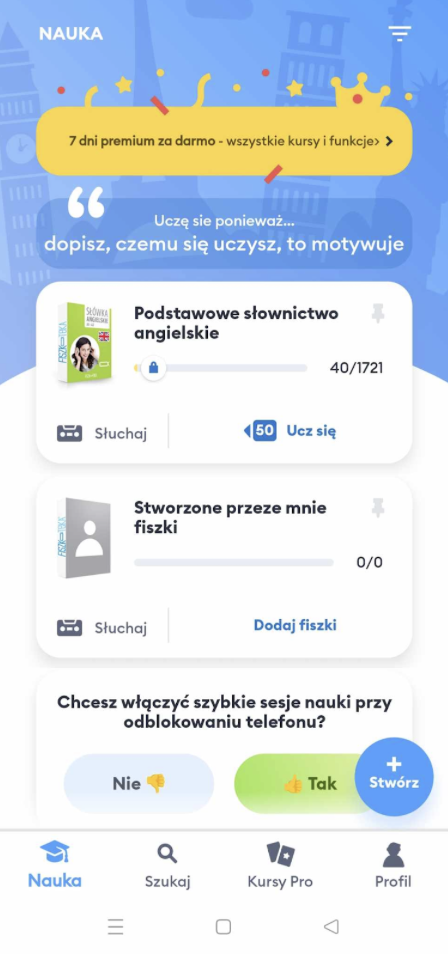
\includegraphics[width=0.3\textwidth]{chapters/chapter_3/fiszoteka.png}
    \caption{Aplikacja mobilna Fiszoteka.}
    \label{img:fiszoteka}
\end{figure}

Zalety:
\begin{itemize}[label=-]
    \item Dostępne talie językowe o różnych poziomach trudności
    \item Odczytanie przez lektora treści fiszki po zobaczeniu odpowiedzi
    \item Tryb słuchania, tytuł i treść fiszek są odczytywane po kolei przez lektora
    \item Dostęp do publicznych talii
    \item Można pobrać dokument PDF lub Mp3 z fiszek
\end{itemize}

Wady:
\begin{itemize}[label=-]
    \item Pełny dostęp do wszystkich funkcjonalności tylko za opłatą
    \item Dla bezpłatnej wersji ograniczenie liczby utworzonych fiszek do 300
    \item Reklamy w aplikacji
    \item Lektor w bezpłatnej wersji ograniczony do 20 dźwięków dziennie
    \item Brak trybu sterowania talii głosem
    \item Aplikacja ukierunkowana na uczenie się słówek
\end{itemize}

\subsection{Gizmo}

Aplikacja wykorzystuje narzędzia sztucznej inteligencji, które pozwalają na tworzenie zestawów fiszek na podstawie plików PDF, CSV lub filmów na platformie YouTube. Gizmo posiada zarówno stronę internetową, jak i aplikację mobilną na Androida i iOS.

\begin{figure}[H]
    \centering
    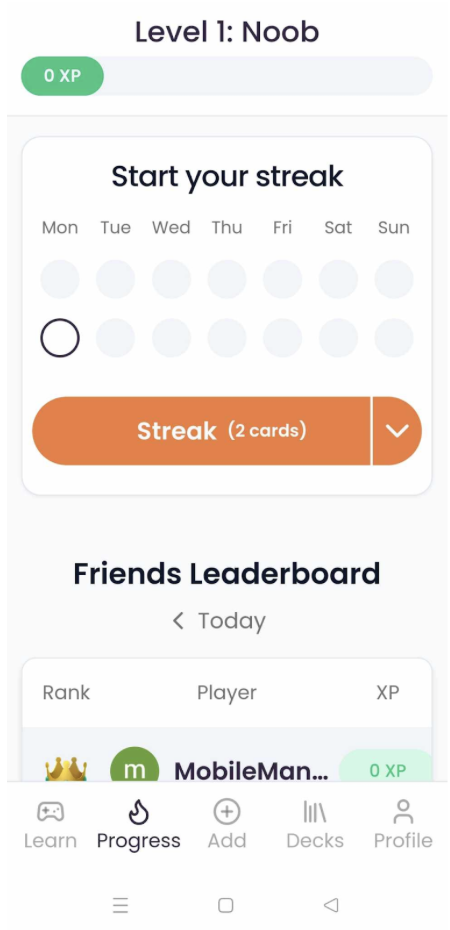
\includegraphics[width=0.3\textwidth]{chapters/chapter_3/gizmo.png}
    \caption{Aplikacja mobilna Gizmo.}
    \label{img:gizmo}
\end{figure}

Zalety:
\begin{itemize}[label=-]
    \item Brak reklam, brak opłat
    \item Zaawansowane zastosowanie AI do tworzenia fiszek
    \item Automatyczne tłumaczenie skanu na język angielski
    \item Szybki i prosty import fiszek z różnych źródeł
    \item Kalendarz passy (streak) zachęcający do nauki
    \item Przejrzysty interfejs
    \item Dostęp do publicznych talii
\end{itemize}

Wady:
\begin{itemize}[label=-]
    \item Nieumiejętne użycie AI przy tworzeniu, prowadzi do utworzenia bezsensownych talii
    \item Dużo niezagospodarowanej przestrzeni na ekranie w trybie uczenia
    \item Brak rankingu popularności talii użytkowników
    \item Domyślnie irytująca częstotliwość powiadomień
    \item Brak trybu sterowania talii głosem
\end{itemize}

\subsection{Flashcards}

Aplikacja dostępna tylko w wersji mobilnej. Ukierunkowana na uczenie się ze słuchu i tworzenie talii z użyciem mowy. Nieintuicyjny interfejs sprawia, że aplikacja jest nieprzyjazna dla nowych użytkowników.

\begin{figure}[H]
    \centering
    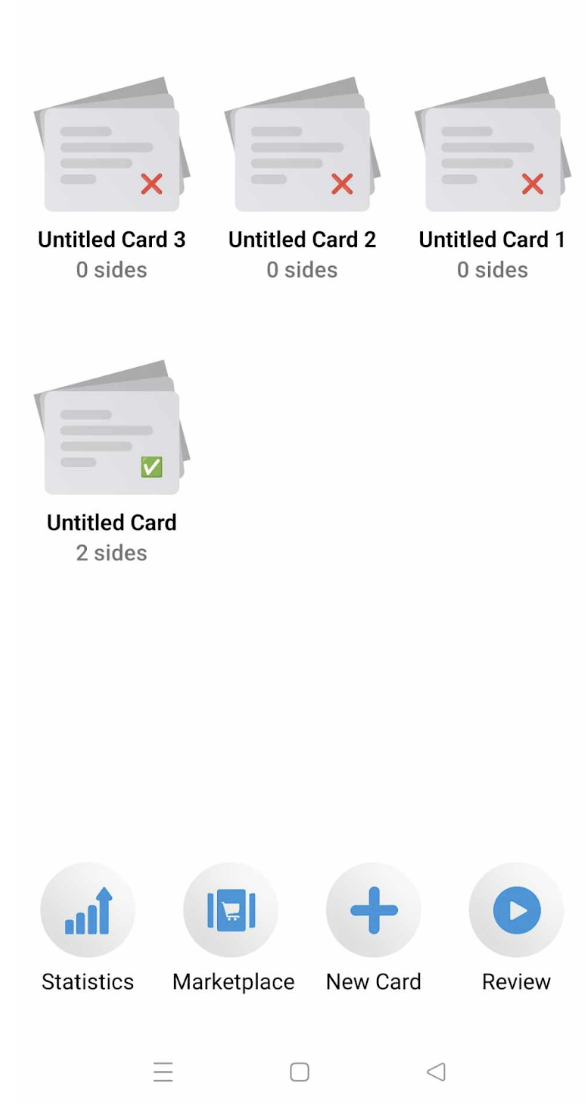
\includegraphics[width=0.3\textwidth]{chapters/chapter_3/flashcards.png}
    \caption{Aplikacja mobilna Flashcards.}
    \label{img:flashcards}
\end{figure}

Zalety:
\begin{itemize}[label=-]
    \item W trybie uczenia pozwala na korzystanie bez dotykania
    \item Możliwość tworzenia fiszek poprzez dyktowanie
    \item Brak reklam, brak opłat
\end{itemize}

Wady:
\begin{itemize}[label=-]
    \item Bardzo archaiczny interfejs
    \item Nieintuicyjny interfejs
    \item Skromna instrukcja korzystania
    \item W trybie uczenia można tylko słuchać i czekać na timer, nie ma nasłuchiwania haseł/komend
    \item Brak publicznych talii
\end{itemize}

\section{Analiza szans oraz zalet względem konkurencyjnych rozwiązań}

Podrozdział zawiera spis najważniejszych funkcjonalności, które odróżniają aplikację fiszki od innych produktów dostępnych na rynku.

\subsection{Szanse/Zalety względem konkurencyjnych rozwiązań}

Zalety:
\begin{itemize}[label=-]
    \item Sterowanie głosowe talii
    \item Generowanie treści fiszki, wykorzystując ChatGPT
    \item Ranking najpopularniejszych talii
\end{itemize}

\subsection{Wady względem konkurencyjnych rozwiązań}

Wady:
\begin{itemize}[label=-]
    \item Aplikacja dostępna tylko w języku angielskim uniemożliwia uczenie się języków obcych
    \item Brak narzędzi generowania zestawów talii z różnych formatów plików takich jak: CSV, mp4, PDF
    \item Brak możliwości generowania testów wielokrotnego wyboru lub prawda/fałsz
    \item Nie można eksportować talii do innych formatów plików takich jak PDF lub CSV
\end{itemize}

\section{Analiza ryzyka}

Podrozdział przedstawia analizę ryzyka, która ma na celu określenie i zrozumienie potencjalnych zagrożeń, które mogą wpłynąć na proces tworzenia projektu.


\newpage

\begin{longtable}{|p{2.3cm}|p{2.3cm}|p{2.3cm}|p{2.3cm}|p{2.3cm}|p{2.3cm}|}
    \hline
\textbf{Zidentyfiko- wane ryzyko [20]} & \textbf{Symptomy} & \textbf{Środki / Działania zapobiegawcze i szacowany poziom trudności ich wdrożenia} & \textbf{Środki / Działania minimalizujące wpływ na projekt – już po jego wystąpieniu i szacowany poziom trudności ich wdrożenia (1-10)} & \textbf{Ranga ryzyka (im niższa, tym mniejszy negatywny wpływ na projekt)} & \textbf{Prawdopodo- bieństwo wystąpienia (1-100\%)} \\
\hline
Błędy w kodzie [O] & Błędy w kompilacji, wyniki testów nie pokrywają się z oczekiwanym rezultatem  & Szybka identyfikacja błędów, wykonywanie testów oprogramowania & Poprawa kodu, testowanie na bieżąco nowo implementowanych funkcjonalności (4) & 10 & 80\% \\
\hline
Awaria sprzętu deweloperskiego [S] & Sprzęt przestaje działać, brak możliwości odzyskania danych & Częste commity na repozytorium & Działanie na ostatniej wersji z repozytorium (1) & 7 & 10\% \\
\hline
Niedobór umiejętności w zespole [L] & Problemy jednostek w poszczególnych zadaniach & Uzupełnianie wiedzy & Pomoc innych członków zespołu (2) & 7 & 70\% \\
\hline
Niezgodność czasowa zespołu [C]  & Osoba blokuje postęp nad projektem poprzez odpowiedzialność nad kluczowym elementem & Wcześniejsze zaplanowanie pracy & Wspólna praca nad kluczowym elementem zajęcie się zadaniami niepowiązanymi (5) & 6 & 80\% \\
\hline
Wybór nieodpowiedniej technologii [T] & Planowane rozwiązania nie są osiągalne przez wykorzystywane technologie & Dogłębna analiza potrzebnych technologii i ich możliwości/ograniczeń & Dopasowanie alternatywnych możliwych rozwiązań (8) & 5 & 50\% \\
\hline
Niedoszacowa- nie budżetu potrzebnego do utrzymania infrastruktury [B] & Budżet zbliża się do wyczerpania przed zaplanowanym terminem  & Analiza cenników wykorzystywanych produktów & Próba pozyskania inwestorów (10) & 10 & 80\% \\
\hline
ChatGPT 3.5 generuje bezsensowną treść dotycząca zagadnienia o którą został zapytany przez użytkownika [F] & Generowane treści nie nawiązują do zagadnienia, o które chat został zapytany & Próba sprecyzowania zapytania, które zostało przesłane do chatu w celu wygenerowania konkretniejszej treści & Użytkownik może zaakceptować lub odrzucić wygenerowaną treść. (4) & 7 & 50\% \\
\hline
    Przeglądarka niepoprawnie wczytuje stronę internetową [Ś] & Style strony nie wyglądają tak samo jak na stronie uruchomionej lokalnie lub na innych przeglądarkach. Pozycje elementów na stronie są inaczej rozmieszczone. & Próba dostosowania styli lub funkcjonalności do konkretnej przeglądarki.  & Uruchomienie strony internetowej na innej przeglądarce (3).   & 10 & 70\% \\
    \hline
\end{longtable}



    \chapter{Projekt w kontekście problemu}

\section{Omówienie zakresu projektu}

W odpowiedzi na zdefiniowany i omówiony w Rozdziale II problem, niniejszy projekt zakłada wytworzenie aplikacji edukacyjnej, która umożliwi naukę metodą wykorzystującą fiszki. Projekt obejmuje dostarczenie aplikacji webowej dostępnej z poziomu przeglądarki internetowej oraz aplikacji mobilnej dla urządzeń z systemem Android lub iOS. W zakres prac wlicza się także zbudowanie pełnej infrastruktury wspierającej aplikację - backend oraz serwer utrzymujący cały system.

\section{Proponowane rozwiązanie}

Projekt bazuje na kilku kluczowych założeniach, które mają na celu bezpośrednie rozwiązanie problemów opisanych w Rozdziale II:

\begin{itemize}
    \item obsługa głosowa: integracja obsługi głosowej aplikacji ma ułatwić korzystanie z niej w sytuacjach, w których użytkownik ma ograniczone możliwości fizycznej obsługi urządzenia. Dzięki temu nauka jest możliwa w każdych warunkach, co odpowiada na problem ograniczonej dostępności tradycyjnych metod nauki;
    \item narzędzie AI do tworzenia fiszek: udostępnienie narzędzia umożliwiającego automatyczne generowanie i dobieranie definicji/odpowiedzi do zagadnień w fiszkach. Pozwala przyśpieszyć i uprzystępnić proces redagowania fiszek.
\end{itemize}

\section{Grupa docelowa}

Główną grupę użytkowników stanowią uczniowie i studenci, a także osoby, które nie mają czasu na tradycyjną formę przyswajania wiedzy, na przykład czytanie lub naukę przy biurku w domowym zaciszu. Generowanie definicji przy użyciu programu ChatGPT pozwala na szybkie tworzenie zestawów fiszek, co może być bardzo wygodne dla osób ceniących sobie czas. Głosowa obsługa talii fiszek pozwala na wykonywanie sesji nauki w warunkach niesprzyjających innym formom uczenia się. Użytkownik ma możliwość powtórzenia materiału, wykonując inne obowiązki, takie jak gotowanie, sprzątanie lub inne czynności, którym nie trzeba poświęcać większej uwagi.

\section{Analiza rozwiązań konkurencji}

Ważnym aspektem tworzenia nowego produktu lub usługi jest analiza konkurencji. Dostrzeżenie wad i zalet konkurencyjnych rozwiązań pozwala na ulepszenie produktów dostępnych na rynku i dotarcie do nowej grupy klientów.

\subsection{Quizlet}

%\putimage{Aplikacja mobilna Quizlet.}{chapters/chapter_3/quizlet.png}{img:quizlet}{0.5\textwidth}

Jedna z pierwszych dostępnych na rynku aplikacja do fiszek. Utworzone w 2005 roku narzędzie do nauki zgromadziło ogromną bazę użytkowników szacowaną na około 50 milionów. Quizlet posiada stronę internetową i aplikacje mobilną dostępne na Android i IOS.

\begin{figure}[H]
    \centering
    
\includegraphics[width=0.3\textwidth]{chapters/chapter_3/quizlet.png}
    \caption{Aplikacja mobilna Quizlet.}
    \label{img:quizlet}
\end{figure}

Zalety:
\begin{itemize}[label=-]
    \item Możliwość tworzenia testów w różnych trybach: prawda/fałsz, wielokrotny wybór, pisemny
    \item Odczytanie przez lektora treści fiszki poprzez kliknięcie przycisku
    \item Dostęp do materiałów, które zostały zweryfikowane przez ekspertów
    \item Personalizacja fiszek za pomocą obrazów i dźwięków
    \item Pozwala na wyszukiwanie talii innych użytkowników
\end{itemize}

Wady:
\begin{itemize}[label=-]
    \item Reklamy w aplikacji
    \item Pełny dostęp do wszystkich funkcjonalności tylko za opłatą
    \item Brak rankingu popularności talii użytkowników, co pozwalałoby na łatwy dostęp do innych talii
    \item Brak trybu sterowania talii głosem
\end{itemize}

\subsection{Fiszkoteka}

Polski portal do nauki metodą fiszek ukierunkowany na naukę języków obcych. Oprócz strony internetowej aplikacja dostępna na system Android lub iOS.

\begin{figure}[H]
    \centering
    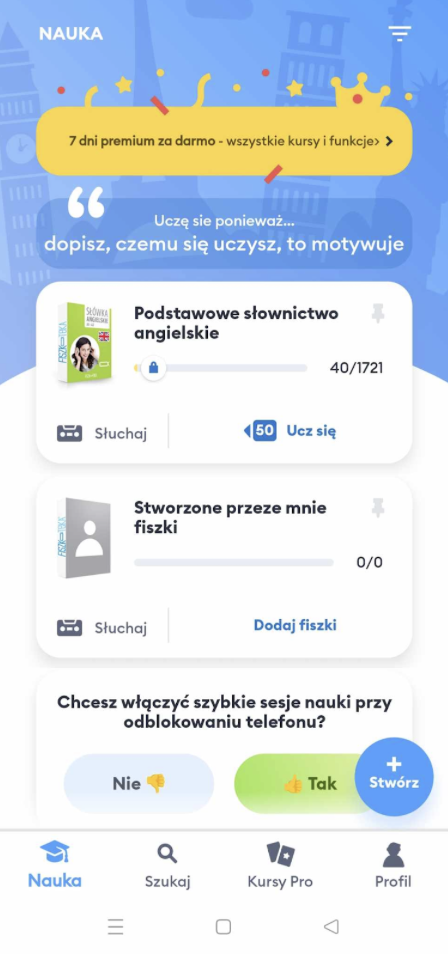
\includegraphics[width=0.3\textwidth]{chapters/chapter_3/fiszoteka.png}
    \caption{Aplikacja mobilna Fiszoteka.}
    \label{img:fiszoteka}
\end{figure}

Zalety:
\begin{itemize}[label=-]
    \item Dostępne talie językowe o różnych poziomach trudności
    \item Odczytanie przez lektora treści fiszki po zobaczeniu odpowiedzi
    \item Tryb słuchania, tytuł i treść fiszek są odczytywane po kolei przez lektora
    \item Dostęp do publicznych talii
    \item Można pobrać dokument PDF lub Mp3 z fiszek
\end{itemize}

Wady:
\begin{itemize}[label=-]
    \item Pełny dostęp do wszystkich funkcjonalności tylko za opłatą
    \item Dla bezpłatnej wersji ograniczenie liczby utworzonych fiszek do 300
    \item Reklamy w aplikacji
    \item Lektor w bezpłatnej wersji ograniczony do 20 dźwięków dziennie
    \item Brak trybu sterowania talii głosem
    \item Aplikacja ukierunkowana na uczenie się słówek
\end{itemize}

\subsection{Gizmo}

Aplikacja wykorzystuje narzędzia sztucznej inteligencji, które pozwalają na tworzenie zestawów fiszek na podstawie plików PDF, CSV lub filmów na platformie YouTube. Gizmo posiada zarówno stronę internetową, jak i aplikację mobilną na Androida i iOS.

\begin{figure}[H]
    \centering
    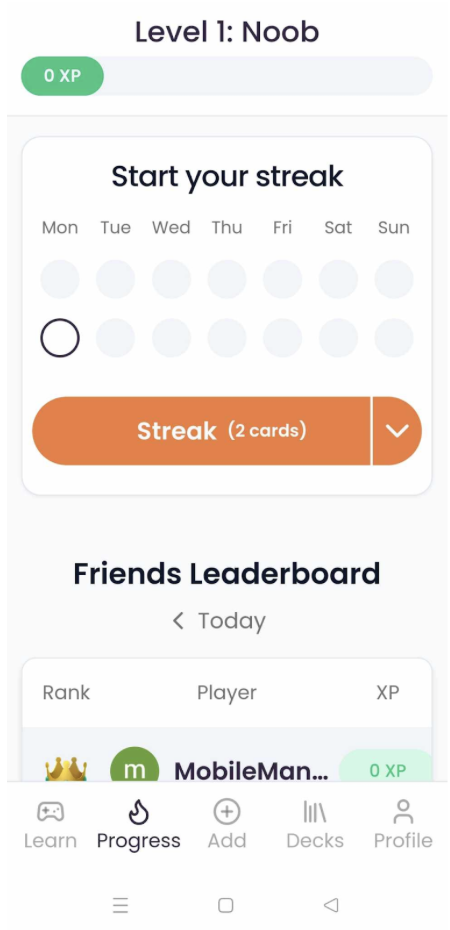
\includegraphics[width=0.3\textwidth]{chapters/chapter_3/gizmo.png}
    \caption{Aplikacja mobilna Gizmo.}
    \label{img:gizmo}
\end{figure}

Zalety:
\begin{itemize}[label=-]
    \item Brak reklam, brak opłat
    \item Zaawansowane zastosowanie AI do tworzenia fiszek
    \item Automatyczne tłumaczenie skanu na język angielski
    \item Szybki i prosty import fiszek z różnych źródeł
    \item Kalendarz passy (streak) zachęcający do nauki
    \item Przejrzysty interfejs
    \item Dostęp do publicznych talii
\end{itemize}

Wady:
\begin{itemize}[label=-]
    \item Nieumiejętne użycie AI przy tworzeniu, prowadzi do utworzenia bezsensownych talii
    \item Dużo niezagospodarowanej przestrzeni na ekranie w trybie uczenia
    \item Brak rankingu popularności talii użytkowników
    \item Domyślnie irytująca częstotliwość powiadomień
    \item Brak trybu sterowania talii głosem
\end{itemize}

\subsection{Flashcards}

Aplikacja dostępna tylko w wersji mobilnej. Ukierunkowana na uczenie się ze słuchu i tworzenie talii z użyciem mowy. Nieintuicyjny interfejs sprawia, że aplikacja jest nieprzyjazna dla nowych użytkowników.

\begin{figure}[H]
    \centering
    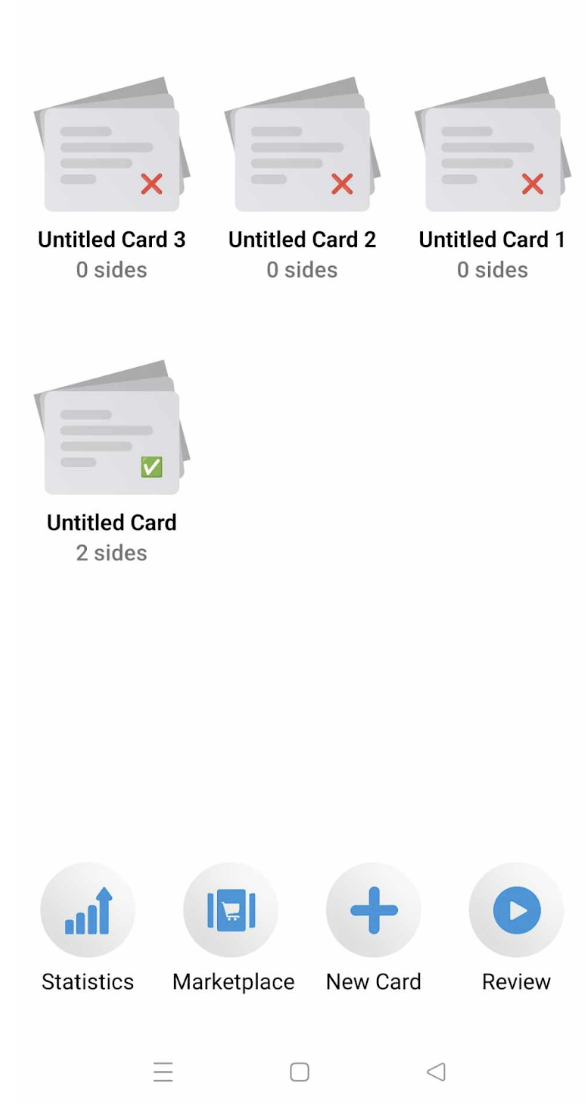
\includegraphics[width=0.3\textwidth]{chapters/chapter_3/flashcards.png}
    \caption{Aplikacja mobilna Flashcards.}
    \label{img:flashcards}
\end{figure}

Zalety:
\begin{itemize}[label=-]
    \item W trybie uczenia pozwala na korzystanie bez dotykania
    \item Możliwość tworzenia fiszek poprzez dyktowanie
    \item Brak reklam, brak opłat
\end{itemize}

Wady:
\begin{itemize}[label=-]
    \item Bardzo archaiczny interfejs
    \item Nieintuicyjny interfejs
    \item Skromna instrukcja korzystania
    \item W trybie uczenia można tylko słuchać i czekać na timer, nie ma nasłuchiwania haseł/komend
    \item Brak publicznych talii
\end{itemize}

\section{Analiza szans oraz zalet względem konkurencyjnych rozwiązań}

Podrozdział zawiera spis najważniejszych funkcjonalności, które odróżniają aplikację fiszki od innych produktów dostępnych na rynku.

\subsection{Szanse/Zalety względem konkurencyjnych rozwiązań}

Zalety:
\begin{itemize}[label=-]
    \item Sterowanie głosowe talii
    \item Generowanie treści fiszki, wykorzystując ChatGPT
    \item Ranking najpopularniejszych talii
\end{itemize}

\subsection{Wady względem konkurencyjnych rozwiązań}

Wady:
\begin{itemize}[label=-]
    \item Aplikacja dostępna tylko w języku angielskim uniemożliwia uczenie się języków obcych
    \item Brak narzędzi generowania zestawów talii z różnych formatów plików takich jak: CSV, mp4, PDF
    \item Brak możliwości generowania testów wielokrotnego wyboru lub prawda/fałsz
    \item Nie można eksportować talii do innych formatów plików takich jak PDF lub CSV
\end{itemize}

\section{Analiza ryzyka}

Podrozdział przedstawia analizę ryzyka, która ma na celu określenie i zrozumienie potencjalnych zagrożeń, które mogą wpłynąć na proces tworzenia projektu.


\newpage

\begin{longtable}{|p{2.3cm}|p{2.3cm}|p{2.3cm}|p{2.3cm}|p{2.3cm}|p{2.3cm}|}
    \hline
\textbf{Zidentyfiko- wane ryzyko [20]} & \textbf{Symptomy} & \textbf{Środki / Działania zapobiegawcze i szacowany poziom trudności ich wdrożenia} & \textbf{Środki / Działania minimalizujące wpływ na projekt – już po jego wystąpieniu i szacowany poziom trudności ich wdrożenia (1-10)} & \textbf{Ranga ryzyka (im niższa, tym mniejszy negatywny wpływ na projekt)} & \textbf{Prawdopodo- bieństwo wystąpienia (1-100\%)} \\
\hline
Błędy w kodzie [O] & Błędy w kompilacji, wyniki testów nie pokrywają się z oczekiwanym rezultatem  & Szybka identyfikacja błędów, wykonywanie testów oprogramowania & Poprawa kodu, testowanie na bieżąco nowo implementowanych funkcjonalności (4) & 10 & 80\% \\
\hline
Awaria sprzętu deweloperskiego [S] & Sprzęt przestaje działać, brak możliwości odzyskania danych & Częste commity na repozytorium & Działanie na ostatniej wersji z repozytorium (1) & 7 & 10\% \\
\hline
Niedobór umiejętności w zespole [L] & Problemy jednostek w poszczególnych zadaniach & Uzupełnianie wiedzy & Pomoc innych członków zespołu (2) & 7 & 70\% \\
\hline
Niezgodność czasowa zespołu [C]  & Osoba blokuje postęp nad projektem poprzez odpowiedzialność nad kluczowym elementem & Wcześniejsze zaplanowanie pracy & Wspólna praca nad kluczowym elementem zajęcie się zadaniami niepowiązanymi (5) & 6 & 80\% \\
\hline
Wybór nieodpowiedniej technologii [T] & Planowane rozwiązania nie są osiągalne przez wykorzystywane technologie & Dogłębna analiza potrzebnych technologii i ich możliwości/ograniczeń & Dopasowanie alternatywnych możliwych rozwiązań (8) & 5 & 50\% \\
\hline
Niedoszacowa- nie budżetu potrzebnego do utrzymania infrastruktury [B] & Budżet zbliża się do wyczerpania przed zaplanowanym terminem  & Analiza cenników wykorzystywanych produktów & Próba pozyskania inwestorów (10) & 10 & 80\% \\
\hline
ChatGPT 3.5 generuje bezsensowną treść dotycząca zagadnienia o którą został zapytany przez użytkownika [F] & Generowane treści nie nawiązują do zagadnienia, o które chat został zapytany & Próba sprecyzowania zapytania, które zostało przesłane do chatu w celu wygenerowania konkretniejszej treści & Użytkownik może zaakceptować lub odrzucić wygenerowaną treść. (4) & 7 & 50\% \\
\hline
    Przeglądarka niepoprawnie wczytuje stronę internetową [Ś] & Style strony nie wyglądają tak samo jak na stronie uruchomionej lokalnie lub na innych przeglądarkach. Pozycje elementów na stronie są inaczej rozmieszczone. & Próba dostosowania styli lub funkcjonalności do konkretnej przeglądarki.  & Uruchomienie strony internetowej na innej przeglądarce (3).   & 10 & 70\% \\
    \hline
\end{longtable}



    \chapter{Projekt w kontekście problemu}

\section{Omówienie zakresu projektu}

W odpowiedzi na zdefiniowany i omówiony w Rozdziale II problem, niniejszy projekt zakłada wytworzenie aplikacji edukacyjnej, która umożliwi naukę metodą wykorzystującą fiszki. Projekt obejmuje dostarczenie aplikacji webowej dostępnej z poziomu przeglądarki internetowej oraz aplikacji mobilnej dla urządzeń z systemem Android lub iOS. W zakres prac wlicza się także zbudowanie pełnej infrastruktury wspierającej aplikację - backend oraz serwer utrzymujący cały system.

\section{Proponowane rozwiązanie}

Projekt bazuje na kilku kluczowych założeniach, które mają na celu bezpośrednie rozwiązanie problemów opisanych w Rozdziale II:

\begin{itemize}
    \item obsługa głosowa: integracja obsługi głosowej aplikacji ma ułatwić korzystanie z niej w sytuacjach, w których użytkownik ma ograniczone możliwości fizycznej obsługi urządzenia. Dzięki temu nauka jest możliwa w każdych warunkach, co odpowiada na problem ograniczonej dostępności tradycyjnych metod nauki;
    \item narzędzie AI do tworzenia fiszek: udostępnienie narzędzia umożliwiającego automatyczne generowanie i dobieranie definicji/odpowiedzi do zagadnień w fiszkach. Pozwala przyśpieszyć i uprzystępnić proces redagowania fiszek.
\end{itemize}

\section{Grupa docelowa}

Główną grupę użytkowników stanowią uczniowie i studenci, a także osoby, które nie mają czasu na tradycyjną formę przyswajania wiedzy, na przykład czytanie lub naukę przy biurku w domowym zaciszu. Generowanie definicji przy użyciu programu ChatGPT pozwala na szybkie tworzenie zestawów fiszek, co może być bardzo wygodne dla osób ceniących sobie czas. Głosowa obsługa talii fiszek pozwala na wykonywanie sesji nauki w warunkach niesprzyjających innym formom uczenia się. Użytkownik ma możliwość powtórzenia materiału, wykonując inne obowiązki, takie jak gotowanie, sprzątanie lub inne czynności, którym nie trzeba poświęcać większej uwagi.

\section{Analiza rozwiązań konkurencji}

Ważnym aspektem tworzenia nowego produktu lub usługi jest analiza konkurencji. Dostrzeżenie wad i zalet konkurencyjnych rozwiązań pozwala na ulepszenie produktów dostępnych na rynku i dotarcie do nowej grupy klientów.

\subsection{Quizlet}

%\putimage{Aplikacja mobilna Quizlet.}{chapters/chapter_3/quizlet.png}{img:quizlet}{0.5\textwidth}

Jedna z pierwszych dostępnych na rynku aplikacja do fiszek. Utworzone w 2005 roku narzędzie do nauki zgromadziło ogromną bazę użytkowników szacowaną na około 50 milionów. Quizlet posiada stronę internetową i aplikacje mobilną dostępne na Android i IOS.

\begin{figure}[H]
    \centering
    
\includegraphics[width=0.3\textwidth]{chapters/chapter_3/quizlet.png}
    \caption{Aplikacja mobilna Quizlet.}
    \label{img:quizlet}
\end{figure}

Zalety:
\begin{itemize}[label=-]
    \item Możliwość tworzenia testów w różnych trybach: prawda/fałsz, wielokrotny wybór, pisemny
    \item Odczytanie przez lektora treści fiszki poprzez kliknięcie przycisku
    \item Dostęp do materiałów, które zostały zweryfikowane przez ekspertów
    \item Personalizacja fiszek za pomocą obrazów i dźwięków
    \item Pozwala na wyszukiwanie talii innych użytkowników
\end{itemize}

Wady:
\begin{itemize}[label=-]
    \item Reklamy w aplikacji
    \item Pełny dostęp do wszystkich funkcjonalności tylko za opłatą
    \item Brak rankingu popularności talii użytkowników, co pozwalałoby na łatwy dostęp do innych talii
    \item Brak trybu sterowania talii głosem
\end{itemize}

\subsection{Fiszkoteka}

Polski portal do nauki metodą fiszek ukierunkowany na naukę języków obcych. Oprócz strony internetowej aplikacja dostępna na system Android lub iOS.

\begin{figure}[H]
    \centering
    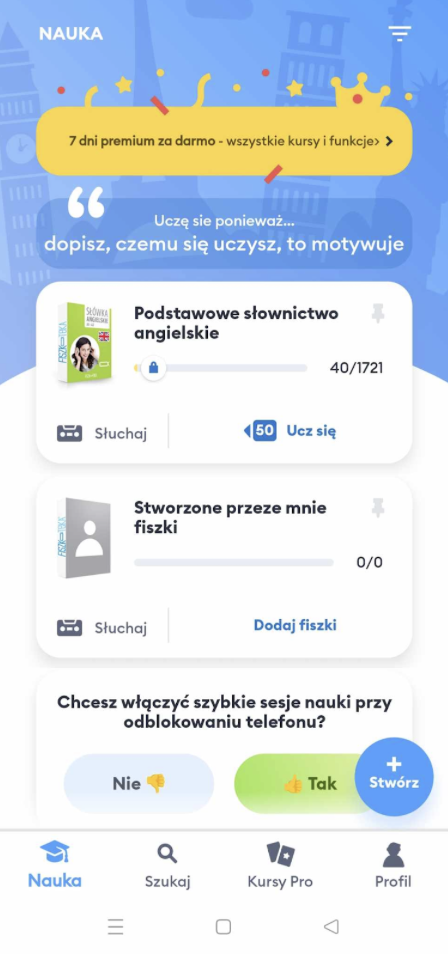
\includegraphics[width=0.3\textwidth]{chapters/chapter_3/fiszoteka.png}
    \caption{Aplikacja mobilna Fiszoteka.}
    \label{img:fiszoteka}
\end{figure}

Zalety:
\begin{itemize}[label=-]
    \item Dostępne talie językowe o różnych poziomach trudności
    \item Odczytanie przez lektora treści fiszki po zobaczeniu odpowiedzi
    \item Tryb słuchania, tytuł i treść fiszek są odczytywane po kolei przez lektora
    \item Dostęp do publicznych talii
    \item Można pobrać dokument PDF lub Mp3 z fiszek
\end{itemize}

Wady:
\begin{itemize}[label=-]
    \item Pełny dostęp do wszystkich funkcjonalności tylko za opłatą
    \item Dla bezpłatnej wersji ograniczenie liczby utworzonych fiszek do 300
    \item Reklamy w aplikacji
    \item Lektor w bezpłatnej wersji ograniczony do 20 dźwięków dziennie
    \item Brak trybu sterowania talii głosem
    \item Aplikacja ukierunkowana na uczenie się słówek
\end{itemize}

\subsection{Gizmo}

Aplikacja wykorzystuje narzędzia sztucznej inteligencji, które pozwalają na tworzenie zestawów fiszek na podstawie plików PDF, CSV lub filmów na platformie YouTube. Gizmo posiada zarówno stronę internetową, jak i aplikację mobilną na Androida i iOS.

\begin{figure}[H]
    \centering
    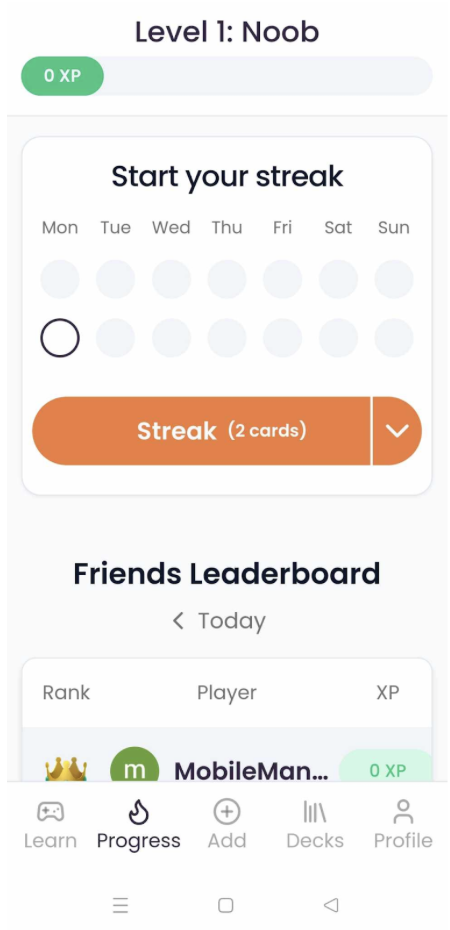
\includegraphics[width=0.3\textwidth]{chapters/chapter_3/gizmo.png}
    \caption{Aplikacja mobilna Gizmo.}
    \label{img:gizmo}
\end{figure}

Zalety:
\begin{itemize}[label=-]
    \item Brak reklam, brak opłat
    \item Zaawansowane zastosowanie AI do tworzenia fiszek
    \item Automatyczne tłumaczenie skanu na język angielski
    \item Szybki i prosty import fiszek z różnych źródeł
    \item Kalendarz passy (streak) zachęcający do nauki
    \item Przejrzysty interfejs
    \item Dostęp do publicznych talii
\end{itemize}

Wady:
\begin{itemize}[label=-]
    \item Nieumiejętne użycie AI przy tworzeniu, prowadzi do utworzenia bezsensownych talii
    \item Dużo niezagospodarowanej przestrzeni na ekranie w trybie uczenia
    \item Brak rankingu popularności talii użytkowników
    \item Domyślnie irytująca częstotliwość powiadomień
    \item Brak trybu sterowania talii głosem
\end{itemize}

\subsection{Flashcards}

Aplikacja dostępna tylko w wersji mobilnej. Ukierunkowana na uczenie się ze słuchu i tworzenie talii z użyciem mowy. Nieintuicyjny interfejs sprawia, że aplikacja jest nieprzyjazna dla nowych użytkowników.

\begin{figure}[H]
    \centering
    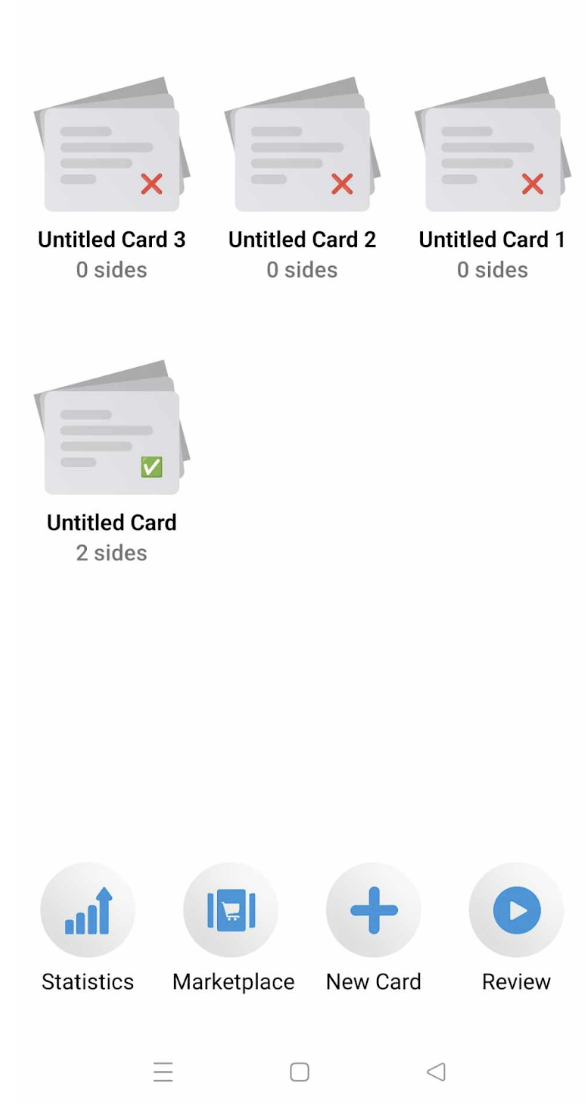
\includegraphics[width=0.3\textwidth]{chapters/chapter_3/flashcards.png}
    \caption{Aplikacja mobilna Flashcards.}
    \label{img:flashcards}
\end{figure}

Zalety:
\begin{itemize}[label=-]
    \item W trybie uczenia pozwala na korzystanie bez dotykania
    \item Możliwość tworzenia fiszek poprzez dyktowanie
    \item Brak reklam, brak opłat
\end{itemize}

Wady:
\begin{itemize}[label=-]
    \item Bardzo archaiczny interfejs
    \item Nieintuicyjny interfejs
    \item Skromna instrukcja korzystania
    \item W trybie uczenia można tylko słuchać i czekać na timer, nie ma nasłuchiwania haseł/komend
    \item Brak publicznych talii
\end{itemize}

\section{Analiza szans oraz zalet względem konkurencyjnych rozwiązań}

Podrozdział zawiera spis najważniejszych funkcjonalności, które odróżniają aplikację fiszki od innych produktów dostępnych na rynku.

\subsection{Szanse/Zalety względem konkurencyjnych rozwiązań}

Zalety:
\begin{itemize}[label=-]
    \item Sterowanie głosowe talii
    \item Generowanie treści fiszki, wykorzystując ChatGPT
    \item Ranking najpopularniejszych talii
\end{itemize}

\subsection{Wady względem konkurencyjnych rozwiązań}

Wady:
\begin{itemize}[label=-]
    \item Aplikacja dostępna tylko w języku angielskim uniemożliwia uczenie się języków obcych
    \item Brak narzędzi generowania zestawów talii z różnych formatów plików takich jak: CSV, mp4, PDF
    \item Brak możliwości generowania testów wielokrotnego wyboru lub prawda/fałsz
    \item Nie można eksportować talii do innych formatów plików takich jak PDF lub CSV
\end{itemize}

\section{Analiza ryzyka}

Podrozdział przedstawia analizę ryzyka, która ma na celu określenie i zrozumienie potencjalnych zagrożeń, które mogą wpłynąć na proces tworzenia projektu.


\newpage

\begin{longtable}{|p{2.3cm}|p{2.3cm}|p{2.3cm}|p{2.3cm}|p{2.3cm}|p{2.3cm}|}
    \hline
\textbf{Zidentyfiko- wane ryzyko [20]} & \textbf{Symptomy} & \textbf{Środki / Działania zapobiegawcze i szacowany poziom trudności ich wdrożenia} & \textbf{Środki / Działania minimalizujące wpływ na projekt – już po jego wystąpieniu i szacowany poziom trudności ich wdrożenia (1-10)} & \textbf{Ranga ryzyka (im niższa, tym mniejszy negatywny wpływ na projekt)} & \textbf{Prawdopodo- bieństwo wystąpienia (1-100\%)} \\
\hline
Błędy w kodzie [O] & Błędy w kompilacji, wyniki testów nie pokrywają się z oczekiwanym rezultatem  & Szybka identyfikacja błędów, wykonywanie testów oprogramowania & Poprawa kodu, testowanie na bieżąco nowo implementowanych funkcjonalności (4) & 10 & 80\% \\
\hline
Awaria sprzętu deweloperskiego [S] & Sprzęt przestaje działać, brak możliwości odzyskania danych & Częste commity na repozytorium & Działanie na ostatniej wersji z repozytorium (1) & 7 & 10\% \\
\hline
Niedobór umiejętności w zespole [L] & Problemy jednostek w poszczególnych zadaniach & Uzupełnianie wiedzy & Pomoc innych członków zespołu (2) & 7 & 70\% \\
\hline
Niezgodność czasowa zespołu [C]  & Osoba blokuje postęp nad projektem poprzez odpowiedzialność nad kluczowym elementem & Wcześniejsze zaplanowanie pracy & Wspólna praca nad kluczowym elementem zajęcie się zadaniami niepowiązanymi (5) & 6 & 80\% \\
\hline
Wybór nieodpowiedniej technologii [T] & Planowane rozwiązania nie są osiągalne przez wykorzystywane technologie & Dogłębna analiza potrzebnych technologii i ich możliwości/ograniczeń & Dopasowanie alternatywnych możliwych rozwiązań (8) & 5 & 50\% \\
\hline
Niedoszacowa- nie budżetu potrzebnego do utrzymania infrastruktury [B] & Budżet zbliża się do wyczerpania przed zaplanowanym terminem  & Analiza cenników wykorzystywanych produktów & Próba pozyskania inwestorów (10) & 10 & 80\% \\
\hline
ChatGPT 3.5 generuje bezsensowną treść dotycząca zagadnienia o którą został zapytany przez użytkownika [F] & Generowane treści nie nawiązują do zagadnienia, o które chat został zapytany & Próba sprecyzowania zapytania, które zostało przesłane do chatu w celu wygenerowania konkretniejszej treści & Użytkownik może zaakceptować lub odrzucić wygenerowaną treść. (4) & 7 & 50\% \\
\hline
    Przeglądarka niepoprawnie wczytuje stronę internetową [Ś] & Style strony nie wyglądają tak samo jak na stronie uruchomionej lokalnie lub na innych przeglądarkach. Pozycje elementów na stronie są inaczej rozmieszczone. & Próba dostosowania styli lub funkcjonalności do konkretnej przeglądarki.  & Uruchomienie strony internetowej na innej przeglądarce (3).   & 10 & 70\% \\
    \hline
\end{longtable}



    \chapter{Projekt w kontekście problemu}

\section{Omówienie zakresu projektu}

W odpowiedzi na zdefiniowany i omówiony w Rozdziale II problem, niniejszy projekt zakłada wytworzenie aplikacji edukacyjnej, która umożliwi naukę metodą wykorzystującą fiszki. Projekt obejmuje dostarczenie aplikacji webowej dostępnej z poziomu przeglądarki internetowej oraz aplikacji mobilnej dla urządzeń z systemem Android lub iOS. W zakres prac wlicza się także zbudowanie pełnej infrastruktury wspierającej aplikację - backend oraz serwer utrzymujący cały system.

\section{Proponowane rozwiązanie}

Projekt bazuje na kilku kluczowych założeniach, które mają na celu bezpośrednie rozwiązanie problemów opisanych w Rozdziale II:

\begin{itemize}
    \item obsługa głosowa: integracja obsługi głosowej aplikacji ma ułatwić korzystanie z niej w sytuacjach, w których użytkownik ma ograniczone możliwości fizycznej obsługi urządzenia. Dzięki temu nauka jest możliwa w każdych warunkach, co odpowiada na problem ograniczonej dostępności tradycyjnych metod nauki;
    \item narzędzie AI do tworzenia fiszek: udostępnienie narzędzia umożliwiającego automatyczne generowanie i dobieranie definicji/odpowiedzi do zagadnień w fiszkach. Pozwala przyśpieszyć i uprzystępnić proces redagowania fiszek.
\end{itemize}

\section{Grupa docelowa}

Główną grupę użytkowników stanowią uczniowie i studenci, a także osoby, które nie mają czasu na tradycyjną formę przyswajania wiedzy, na przykład czytanie lub naukę przy biurku w domowym zaciszu. Generowanie definicji przy użyciu programu ChatGPT pozwala na szybkie tworzenie zestawów fiszek, co może być bardzo wygodne dla osób ceniących sobie czas. Głosowa obsługa talii fiszek pozwala na wykonywanie sesji nauki w warunkach niesprzyjających innym formom uczenia się. Użytkownik ma możliwość powtórzenia materiału, wykonując inne obowiązki, takie jak gotowanie, sprzątanie lub inne czynności, którym nie trzeba poświęcać większej uwagi.

\section{Analiza rozwiązań konkurencji}

Ważnym aspektem tworzenia nowego produktu lub usługi jest analiza konkurencji. Dostrzeżenie wad i zalet konkurencyjnych rozwiązań pozwala na ulepszenie produktów dostępnych na rynku i dotarcie do nowej grupy klientów.

\subsection{Quizlet}

%\putimage{Aplikacja mobilna Quizlet.}{chapters/chapter_3/quizlet.png}{img:quizlet}{0.5\textwidth}

Jedna z pierwszych dostępnych na rynku aplikacja do fiszek. Utworzone w 2005 roku narzędzie do nauki zgromadziło ogromną bazę użytkowników szacowaną na około 50 milionów. Quizlet posiada stronę internetową i aplikacje mobilną dostępne na Android i IOS.

\begin{figure}[H]
    \centering
    
\includegraphics[width=0.3\textwidth]{chapters/chapter_3/quizlet.png}
    \caption{Aplikacja mobilna Quizlet.}
    \label{img:quizlet}
\end{figure}

Zalety:
\begin{itemize}[label=-]
    \item Możliwość tworzenia testów w różnych trybach: prawda/fałsz, wielokrotny wybór, pisemny
    \item Odczytanie przez lektora treści fiszki poprzez kliknięcie przycisku
    \item Dostęp do materiałów, które zostały zweryfikowane przez ekspertów
    \item Personalizacja fiszek za pomocą obrazów i dźwięków
    \item Pozwala na wyszukiwanie talii innych użytkowników
\end{itemize}

Wady:
\begin{itemize}[label=-]
    \item Reklamy w aplikacji
    \item Pełny dostęp do wszystkich funkcjonalności tylko za opłatą
    \item Brak rankingu popularności talii użytkowników, co pozwalałoby na łatwy dostęp do innych talii
    \item Brak trybu sterowania talii głosem
\end{itemize}

\subsection{Fiszkoteka}

Polski portal do nauki metodą fiszek ukierunkowany na naukę języków obcych. Oprócz strony internetowej aplikacja dostępna na system Android lub iOS.

\begin{figure}[H]
    \centering
    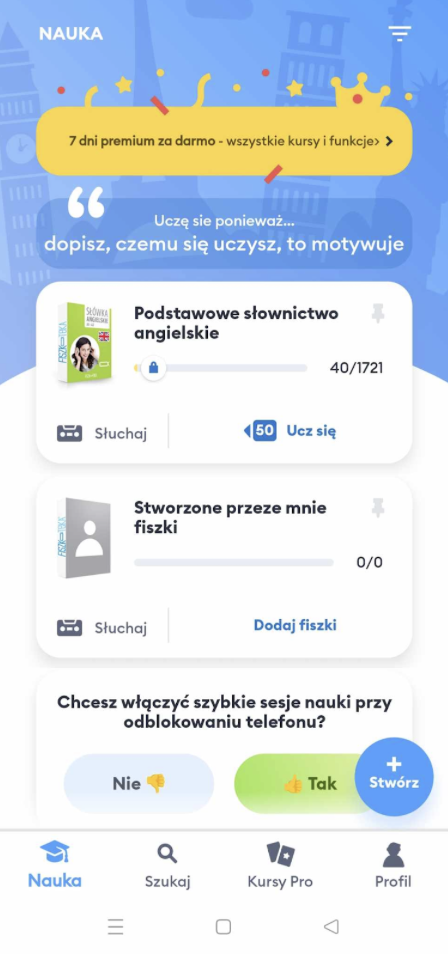
\includegraphics[width=0.3\textwidth]{chapters/chapter_3/fiszoteka.png}
    \caption{Aplikacja mobilna Fiszoteka.}
    \label{img:fiszoteka}
\end{figure}

Zalety:
\begin{itemize}[label=-]
    \item Dostępne talie językowe o różnych poziomach trudności
    \item Odczytanie przez lektora treści fiszki po zobaczeniu odpowiedzi
    \item Tryb słuchania, tytuł i treść fiszek są odczytywane po kolei przez lektora
    \item Dostęp do publicznych talii
    \item Można pobrać dokument PDF lub Mp3 z fiszek
\end{itemize}

Wady:
\begin{itemize}[label=-]
    \item Pełny dostęp do wszystkich funkcjonalności tylko za opłatą
    \item Dla bezpłatnej wersji ograniczenie liczby utworzonych fiszek do 300
    \item Reklamy w aplikacji
    \item Lektor w bezpłatnej wersji ograniczony do 20 dźwięków dziennie
    \item Brak trybu sterowania talii głosem
    \item Aplikacja ukierunkowana na uczenie się słówek
\end{itemize}

\subsection{Gizmo}

Aplikacja wykorzystuje narzędzia sztucznej inteligencji, które pozwalają na tworzenie zestawów fiszek na podstawie plików PDF, CSV lub filmów na platformie YouTube. Gizmo posiada zarówno stronę internetową, jak i aplikację mobilną na Androida i iOS.

\begin{figure}[H]
    \centering
    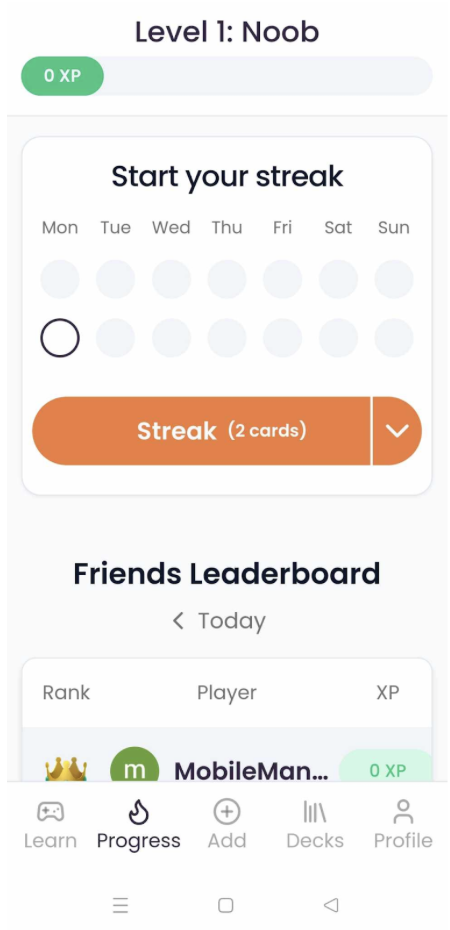
\includegraphics[width=0.3\textwidth]{chapters/chapter_3/gizmo.png}
    \caption{Aplikacja mobilna Gizmo.}
    \label{img:gizmo}
\end{figure}

Zalety:
\begin{itemize}[label=-]
    \item Brak reklam, brak opłat
    \item Zaawansowane zastosowanie AI do tworzenia fiszek
    \item Automatyczne tłumaczenie skanu na język angielski
    \item Szybki i prosty import fiszek z różnych źródeł
    \item Kalendarz passy (streak) zachęcający do nauki
    \item Przejrzysty interfejs
    \item Dostęp do publicznych talii
\end{itemize}

Wady:
\begin{itemize}[label=-]
    \item Nieumiejętne użycie AI przy tworzeniu, prowadzi do utworzenia bezsensownych talii
    \item Dużo niezagospodarowanej przestrzeni na ekranie w trybie uczenia
    \item Brak rankingu popularności talii użytkowników
    \item Domyślnie irytująca częstotliwość powiadomień
    \item Brak trybu sterowania talii głosem
\end{itemize}

\subsection{Flashcards}

Aplikacja dostępna tylko w wersji mobilnej. Ukierunkowana na uczenie się ze słuchu i tworzenie talii z użyciem mowy. Nieintuicyjny interfejs sprawia, że aplikacja jest nieprzyjazna dla nowych użytkowników.

\begin{figure}[H]
    \centering
    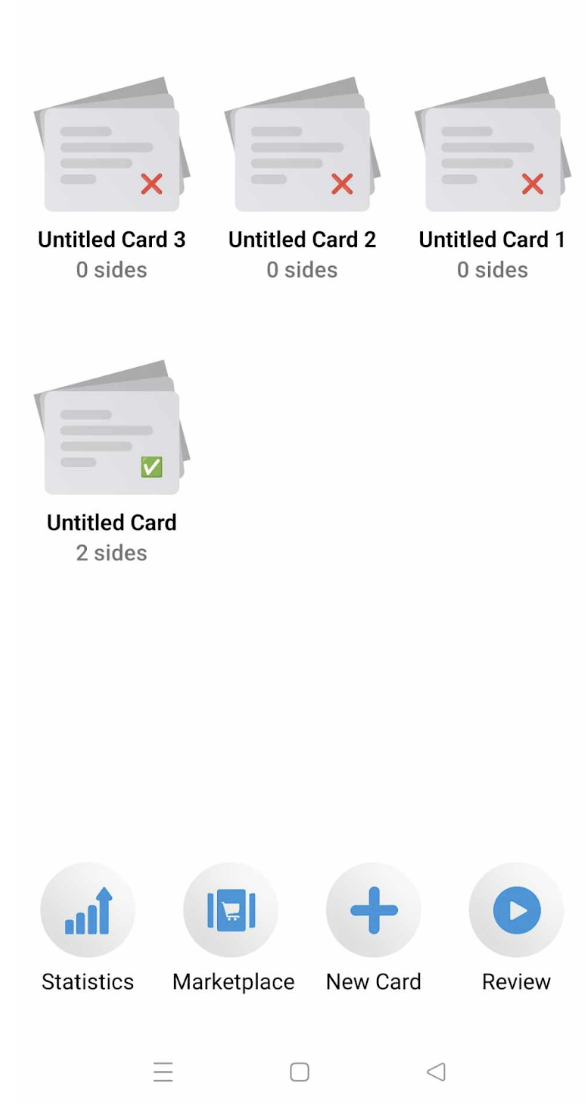
\includegraphics[width=0.3\textwidth]{chapters/chapter_3/flashcards.png}
    \caption{Aplikacja mobilna Flashcards.}
    \label{img:flashcards}
\end{figure}

Zalety:
\begin{itemize}[label=-]
    \item W trybie uczenia pozwala na korzystanie bez dotykania
    \item Możliwość tworzenia fiszek poprzez dyktowanie
    \item Brak reklam, brak opłat
\end{itemize}

Wady:
\begin{itemize}[label=-]
    \item Bardzo archaiczny interfejs
    \item Nieintuicyjny interfejs
    \item Skromna instrukcja korzystania
    \item W trybie uczenia można tylko słuchać i czekać na timer, nie ma nasłuchiwania haseł/komend
    \item Brak publicznych talii
\end{itemize}

\section{Analiza szans oraz zalet względem konkurencyjnych rozwiązań}

Podrozdział zawiera spis najważniejszych funkcjonalności, które odróżniają aplikację fiszki od innych produktów dostępnych na rynku.

\subsection{Szanse/Zalety względem konkurencyjnych rozwiązań}

Zalety:
\begin{itemize}[label=-]
    \item Sterowanie głosowe talii
    \item Generowanie treści fiszki, wykorzystując ChatGPT
    \item Ranking najpopularniejszych talii
\end{itemize}

\subsection{Wady względem konkurencyjnych rozwiązań}

Wady:
\begin{itemize}[label=-]
    \item Aplikacja dostępna tylko w języku angielskim uniemożliwia uczenie się języków obcych
    \item Brak narzędzi generowania zestawów talii z różnych formatów plików takich jak: CSV, mp4, PDF
    \item Brak możliwości generowania testów wielokrotnego wyboru lub prawda/fałsz
    \item Nie można eksportować talii do innych formatów plików takich jak PDF lub CSV
\end{itemize}

\section{Analiza ryzyka}

Podrozdział przedstawia analizę ryzyka, która ma na celu określenie i zrozumienie potencjalnych zagrożeń, które mogą wpłynąć na proces tworzenia projektu.


\newpage

\begin{longtable}{|p{2.3cm}|p{2.3cm}|p{2.3cm}|p{2.3cm}|p{2.3cm}|p{2.3cm}|}
    \hline
\textbf{Zidentyfiko- wane ryzyko [20]} & \textbf{Symptomy} & \textbf{Środki / Działania zapobiegawcze i szacowany poziom trudności ich wdrożenia} & \textbf{Środki / Działania minimalizujące wpływ na projekt – już po jego wystąpieniu i szacowany poziom trudności ich wdrożenia (1-10)} & \textbf{Ranga ryzyka (im niższa, tym mniejszy negatywny wpływ na projekt)} & \textbf{Prawdopodo- bieństwo wystąpienia (1-100\%)} \\
\hline
Błędy w kodzie [O] & Błędy w kompilacji, wyniki testów nie pokrywają się z oczekiwanym rezultatem  & Szybka identyfikacja błędów, wykonywanie testów oprogramowania & Poprawa kodu, testowanie na bieżąco nowo implementowanych funkcjonalności (4) & 10 & 80\% \\
\hline
Awaria sprzętu deweloperskiego [S] & Sprzęt przestaje działać, brak możliwości odzyskania danych & Częste commity na repozytorium & Działanie na ostatniej wersji z repozytorium (1) & 7 & 10\% \\
\hline
Niedobór umiejętności w zespole [L] & Problemy jednostek w poszczególnych zadaniach & Uzupełnianie wiedzy & Pomoc innych członków zespołu (2) & 7 & 70\% \\
\hline
Niezgodność czasowa zespołu [C]  & Osoba blokuje postęp nad projektem poprzez odpowiedzialność nad kluczowym elementem & Wcześniejsze zaplanowanie pracy & Wspólna praca nad kluczowym elementem zajęcie się zadaniami niepowiązanymi (5) & 6 & 80\% \\
\hline
Wybór nieodpowiedniej technologii [T] & Planowane rozwiązania nie są osiągalne przez wykorzystywane technologie & Dogłębna analiza potrzebnych technologii i ich możliwości/ograniczeń & Dopasowanie alternatywnych możliwych rozwiązań (8) & 5 & 50\% \\
\hline
Niedoszacowa- nie budżetu potrzebnego do utrzymania infrastruktury [B] & Budżet zbliża się do wyczerpania przed zaplanowanym terminem  & Analiza cenników wykorzystywanych produktów & Próba pozyskania inwestorów (10) & 10 & 80\% \\
\hline
ChatGPT 3.5 generuje bezsensowną treść dotycząca zagadnienia o którą został zapytany przez użytkownika [F] & Generowane treści nie nawiązują do zagadnienia, o które chat został zapytany & Próba sprecyzowania zapytania, które zostało przesłane do chatu w celu wygenerowania konkretniejszej treści & Użytkownik może zaakceptować lub odrzucić wygenerowaną treść. (4) & 7 & 50\% \\
\hline
    Przeglądarka niepoprawnie wczytuje stronę internetową [Ś] & Style strony nie wyglądają tak samo jak na stronie uruchomionej lokalnie lub na innych przeglądarkach. Pozycje elementów na stronie są inaczej rozmieszczone. & Próba dostosowania styli lub funkcjonalności do konkretnej przeglądarki.  & Uruchomienie strony internetowej na innej przeglądarce (3).   & 10 & 70\% \\
    \hline
\end{longtable}



    \chapter{Projekt w kontekście problemu}

\section{Omówienie zakresu projektu}

W odpowiedzi na zdefiniowany i omówiony w Rozdziale II problem, niniejszy projekt zakłada wytworzenie aplikacji edukacyjnej, która umożliwi naukę metodą wykorzystującą fiszki. Projekt obejmuje dostarczenie aplikacji webowej dostępnej z poziomu przeglądarki internetowej oraz aplikacji mobilnej dla urządzeń z systemem Android lub iOS. W zakres prac wlicza się także zbudowanie pełnej infrastruktury wspierającej aplikację - backend oraz serwer utrzymujący cały system.

\section{Proponowane rozwiązanie}

Projekt bazuje na kilku kluczowych założeniach, które mają na celu bezpośrednie rozwiązanie problemów opisanych w Rozdziale II:

\begin{itemize}
    \item obsługa głosowa: integracja obsługi głosowej aplikacji ma ułatwić korzystanie z niej w sytuacjach, w których użytkownik ma ograniczone możliwości fizycznej obsługi urządzenia. Dzięki temu nauka jest możliwa w każdych warunkach, co odpowiada na problem ograniczonej dostępności tradycyjnych metod nauki;
    \item narzędzie AI do tworzenia fiszek: udostępnienie narzędzia umożliwiającego automatyczne generowanie i dobieranie definicji/odpowiedzi do zagadnień w fiszkach. Pozwala przyśpieszyć i uprzystępnić proces redagowania fiszek.
\end{itemize}

\section{Grupa docelowa}

Główną grupę użytkowników stanowią uczniowie i studenci, a także osoby, które nie mają czasu na tradycyjną formę przyswajania wiedzy, na przykład czytanie lub naukę przy biurku w domowym zaciszu. Generowanie definicji przy użyciu programu ChatGPT pozwala na szybkie tworzenie zestawów fiszek, co może być bardzo wygodne dla osób ceniących sobie czas. Głosowa obsługa talii fiszek pozwala na wykonywanie sesji nauki w warunkach niesprzyjających innym formom uczenia się. Użytkownik ma możliwość powtórzenia materiału, wykonując inne obowiązki, takie jak gotowanie, sprzątanie lub inne czynności, którym nie trzeba poświęcać większej uwagi.

\section{Analiza rozwiązań konkurencji}

Ważnym aspektem tworzenia nowego produktu lub usługi jest analiza konkurencji. Dostrzeżenie wad i zalet konkurencyjnych rozwiązań pozwala na ulepszenie produktów dostępnych na rynku i dotarcie do nowej grupy klientów.

\subsection{Quizlet}

%\putimage{Aplikacja mobilna Quizlet.}{chapters/chapter_3/quizlet.png}{img:quizlet}{0.5\textwidth}

Jedna z pierwszych dostępnych na rynku aplikacja do fiszek. Utworzone w 2005 roku narzędzie do nauki zgromadziło ogromną bazę użytkowników szacowaną na około 50 milionów. Quizlet posiada stronę internetową i aplikacje mobilną dostępne na Android i IOS.

\begin{figure}[H]
    \centering
    
\includegraphics[width=0.3\textwidth]{chapters/chapter_3/quizlet.png}
    \caption{Aplikacja mobilna Quizlet.}
    \label{img:quizlet}
\end{figure}

Zalety:
\begin{itemize}[label=-]
    \item Możliwość tworzenia testów w różnych trybach: prawda/fałsz, wielokrotny wybór, pisemny
    \item Odczytanie przez lektora treści fiszki poprzez kliknięcie przycisku
    \item Dostęp do materiałów, które zostały zweryfikowane przez ekspertów
    \item Personalizacja fiszek za pomocą obrazów i dźwięków
    \item Pozwala na wyszukiwanie talii innych użytkowników
\end{itemize}

Wady:
\begin{itemize}[label=-]
    \item Reklamy w aplikacji
    \item Pełny dostęp do wszystkich funkcjonalności tylko za opłatą
    \item Brak rankingu popularności talii użytkowników, co pozwalałoby na łatwy dostęp do innych talii
    \item Brak trybu sterowania talii głosem
\end{itemize}

\subsection{Fiszkoteka}

Polski portal do nauki metodą fiszek ukierunkowany na naukę języków obcych. Oprócz strony internetowej aplikacja dostępna na system Android lub iOS.

\begin{figure}[H]
    \centering
    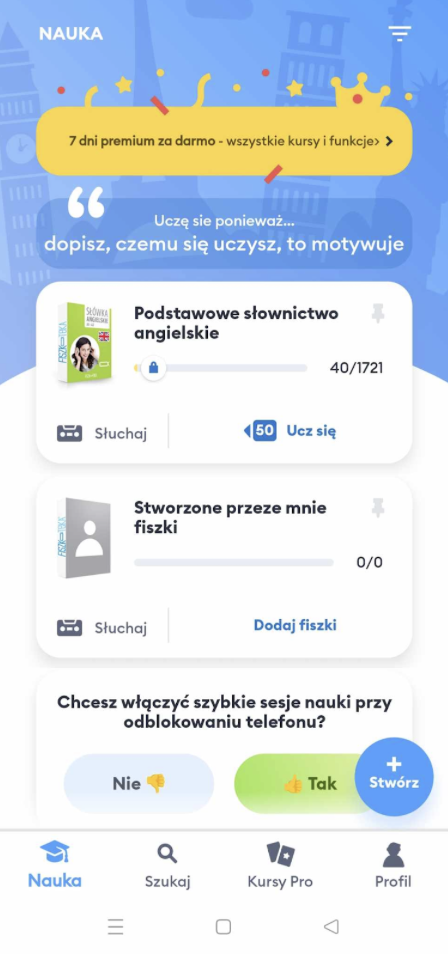
\includegraphics[width=0.3\textwidth]{chapters/chapter_3/fiszoteka.png}
    \caption{Aplikacja mobilna Fiszoteka.}
    \label{img:fiszoteka}
\end{figure}

Zalety:
\begin{itemize}[label=-]
    \item Dostępne talie językowe o różnych poziomach trudności
    \item Odczytanie przez lektora treści fiszki po zobaczeniu odpowiedzi
    \item Tryb słuchania, tytuł i treść fiszek są odczytywane po kolei przez lektora
    \item Dostęp do publicznych talii
    \item Można pobrać dokument PDF lub Mp3 z fiszek
\end{itemize}

Wady:
\begin{itemize}[label=-]
    \item Pełny dostęp do wszystkich funkcjonalności tylko za opłatą
    \item Dla bezpłatnej wersji ograniczenie liczby utworzonych fiszek do 300
    \item Reklamy w aplikacji
    \item Lektor w bezpłatnej wersji ograniczony do 20 dźwięków dziennie
    \item Brak trybu sterowania talii głosem
    \item Aplikacja ukierunkowana na uczenie się słówek
\end{itemize}

\subsection{Gizmo}

Aplikacja wykorzystuje narzędzia sztucznej inteligencji, które pozwalają na tworzenie zestawów fiszek na podstawie plików PDF, CSV lub filmów na platformie YouTube. Gizmo posiada zarówno stronę internetową, jak i aplikację mobilną na Androida i iOS.

\begin{figure}[H]
    \centering
    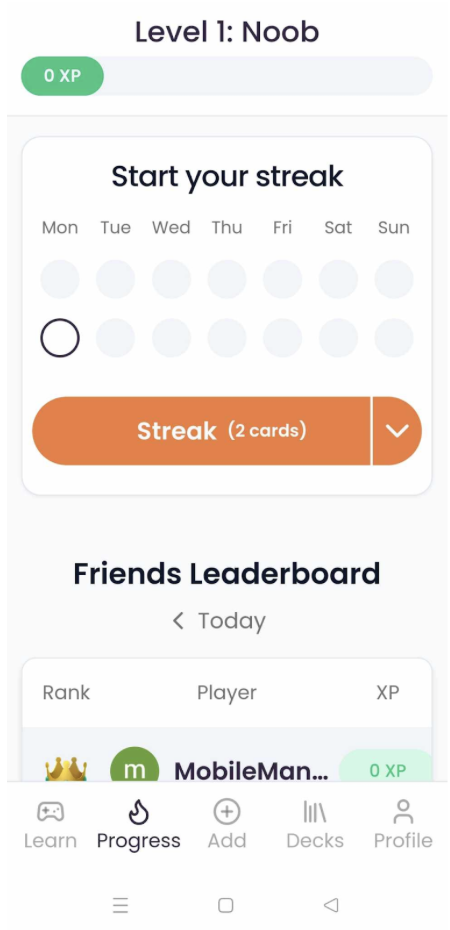
\includegraphics[width=0.3\textwidth]{chapters/chapter_3/gizmo.png}
    \caption{Aplikacja mobilna Gizmo.}
    \label{img:gizmo}
\end{figure}

Zalety:
\begin{itemize}[label=-]
    \item Brak reklam, brak opłat
    \item Zaawansowane zastosowanie AI do tworzenia fiszek
    \item Automatyczne tłumaczenie skanu na język angielski
    \item Szybki i prosty import fiszek z różnych źródeł
    \item Kalendarz passy (streak) zachęcający do nauki
    \item Przejrzysty interfejs
    \item Dostęp do publicznych talii
\end{itemize}

Wady:
\begin{itemize}[label=-]
    \item Nieumiejętne użycie AI przy tworzeniu, prowadzi do utworzenia bezsensownych talii
    \item Dużo niezagospodarowanej przestrzeni na ekranie w trybie uczenia
    \item Brak rankingu popularności talii użytkowników
    \item Domyślnie irytująca częstotliwość powiadomień
    \item Brak trybu sterowania talii głosem
\end{itemize}

\subsection{Flashcards}

Aplikacja dostępna tylko w wersji mobilnej. Ukierunkowana na uczenie się ze słuchu i tworzenie talii z użyciem mowy. Nieintuicyjny interfejs sprawia, że aplikacja jest nieprzyjazna dla nowych użytkowników.

\begin{figure}[H]
    \centering
    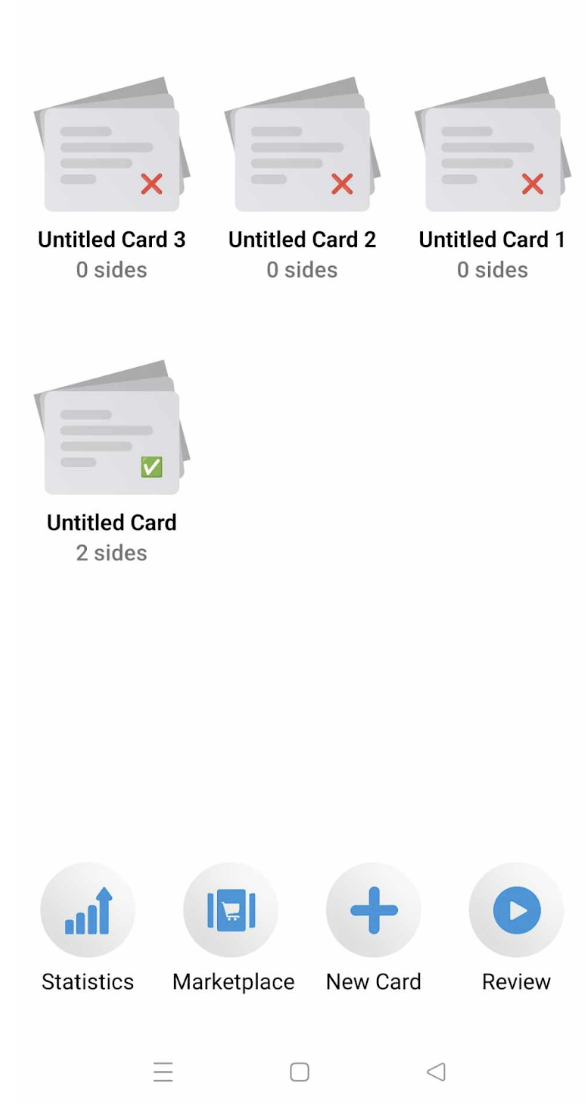
\includegraphics[width=0.3\textwidth]{chapters/chapter_3/flashcards.png}
    \caption{Aplikacja mobilna Flashcards.}
    \label{img:flashcards}
\end{figure}

Zalety:
\begin{itemize}[label=-]
    \item W trybie uczenia pozwala na korzystanie bez dotykania
    \item Możliwość tworzenia fiszek poprzez dyktowanie
    \item Brak reklam, brak opłat
\end{itemize}

Wady:
\begin{itemize}[label=-]
    \item Bardzo archaiczny interfejs
    \item Nieintuicyjny interfejs
    \item Skromna instrukcja korzystania
    \item W trybie uczenia można tylko słuchać i czekać na timer, nie ma nasłuchiwania haseł/komend
    \item Brak publicznych talii
\end{itemize}

\section{Analiza szans oraz zalet względem konkurencyjnych rozwiązań}

Podrozdział zawiera spis najważniejszych funkcjonalności, które odróżniają aplikację fiszki od innych produktów dostępnych na rynku.

\subsection{Szanse/Zalety względem konkurencyjnych rozwiązań}

Zalety:
\begin{itemize}[label=-]
    \item Sterowanie głosowe talii
    \item Generowanie treści fiszki, wykorzystując ChatGPT
    \item Ranking najpopularniejszych talii
\end{itemize}

\subsection{Wady względem konkurencyjnych rozwiązań}

Wady:
\begin{itemize}[label=-]
    \item Aplikacja dostępna tylko w języku angielskim uniemożliwia uczenie się języków obcych
    \item Brak narzędzi generowania zestawów talii z różnych formatów plików takich jak: CSV, mp4, PDF
    \item Brak możliwości generowania testów wielokrotnego wyboru lub prawda/fałsz
    \item Nie można eksportować talii do innych formatów plików takich jak PDF lub CSV
\end{itemize}

\section{Analiza ryzyka}

Podrozdział przedstawia analizę ryzyka, która ma na celu określenie i zrozumienie potencjalnych zagrożeń, które mogą wpłynąć na proces tworzenia projektu.


\newpage

\begin{longtable}{|p{2.3cm}|p{2.3cm}|p{2.3cm}|p{2.3cm}|p{2.3cm}|p{2.3cm}|}
    \hline
\textbf{Zidentyfiko- wane ryzyko [20]} & \textbf{Symptomy} & \textbf{Środki / Działania zapobiegawcze i szacowany poziom trudności ich wdrożenia} & \textbf{Środki / Działania minimalizujące wpływ na projekt – już po jego wystąpieniu i szacowany poziom trudności ich wdrożenia (1-10)} & \textbf{Ranga ryzyka (im niższa, tym mniejszy negatywny wpływ na projekt)} & \textbf{Prawdopodo- bieństwo wystąpienia (1-100\%)} \\
\hline
Błędy w kodzie [O] & Błędy w kompilacji, wyniki testów nie pokrywają się z oczekiwanym rezultatem  & Szybka identyfikacja błędów, wykonywanie testów oprogramowania & Poprawa kodu, testowanie na bieżąco nowo implementowanych funkcjonalności (4) & 10 & 80\% \\
\hline
Awaria sprzętu deweloperskiego [S] & Sprzęt przestaje działać, brak możliwości odzyskania danych & Częste commity na repozytorium & Działanie na ostatniej wersji z repozytorium (1) & 7 & 10\% \\
\hline
Niedobór umiejętności w zespole [L] & Problemy jednostek w poszczególnych zadaniach & Uzupełnianie wiedzy & Pomoc innych członków zespołu (2) & 7 & 70\% \\
\hline
Niezgodność czasowa zespołu [C]  & Osoba blokuje postęp nad projektem poprzez odpowiedzialność nad kluczowym elementem & Wcześniejsze zaplanowanie pracy & Wspólna praca nad kluczowym elementem zajęcie się zadaniami niepowiązanymi (5) & 6 & 80\% \\
\hline
Wybór nieodpowiedniej technologii [T] & Planowane rozwiązania nie są osiągalne przez wykorzystywane technologie & Dogłębna analiza potrzebnych technologii i ich możliwości/ograniczeń & Dopasowanie alternatywnych możliwych rozwiązań (8) & 5 & 50\% \\
\hline
Niedoszacowa- nie budżetu potrzebnego do utrzymania infrastruktury [B] & Budżet zbliża się do wyczerpania przed zaplanowanym terminem  & Analiza cenników wykorzystywanych produktów & Próba pozyskania inwestorów (10) & 10 & 80\% \\
\hline
ChatGPT 3.5 generuje bezsensowną treść dotycząca zagadnienia o którą został zapytany przez użytkownika [F] & Generowane treści nie nawiązują do zagadnienia, o które chat został zapytany & Próba sprecyzowania zapytania, które zostało przesłane do chatu w celu wygenerowania konkretniejszej treści & Użytkownik może zaakceptować lub odrzucić wygenerowaną treść. (4) & 7 & 50\% \\
\hline
    Przeglądarka niepoprawnie wczytuje stronę internetową [Ś] & Style strony nie wyglądają tak samo jak na stronie uruchomionej lokalnie lub na innych przeglądarkach. Pozycje elementów na stronie są inaczej rozmieszczone. & Próba dostosowania styli lub funkcjonalności do konkretnej przeglądarki.  & Uruchomienie strony internetowej na innej przeglądarce (3).   & 10 & 70\% \\
    \hline
\end{longtable}



    \chapter{Projekt w kontekście problemu}

\section{Omówienie zakresu projektu}

W odpowiedzi na zdefiniowany i omówiony w Rozdziale II problem, niniejszy projekt zakłada wytworzenie aplikacji edukacyjnej, która umożliwi naukę metodą wykorzystującą fiszki. Projekt obejmuje dostarczenie aplikacji webowej dostępnej z poziomu przeglądarki internetowej oraz aplikacji mobilnej dla urządzeń z systemem Android lub iOS. W zakres prac wlicza się także zbudowanie pełnej infrastruktury wspierającej aplikację - backend oraz serwer utrzymujący cały system.

\section{Proponowane rozwiązanie}

Projekt bazuje na kilku kluczowych założeniach, które mają na celu bezpośrednie rozwiązanie problemów opisanych w Rozdziale II:

\begin{itemize}
    \item obsługa głosowa: integracja obsługi głosowej aplikacji ma ułatwić korzystanie z niej w sytuacjach, w których użytkownik ma ograniczone możliwości fizycznej obsługi urządzenia. Dzięki temu nauka jest możliwa w każdych warunkach, co odpowiada na problem ograniczonej dostępności tradycyjnych metod nauki;
    \item narzędzie AI do tworzenia fiszek: udostępnienie narzędzia umożliwiającego automatyczne generowanie i dobieranie definicji/odpowiedzi do zagadnień w fiszkach. Pozwala przyśpieszyć i uprzystępnić proces redagowania fiszek.
\end{itemize}

\section{Grupa docelowa}

Główną grupę użytkowników stanowią uczniowie i studenci, a także osoby, które nie mają czasu na tradycyjną formę przyswajania wiedzy, na przykład czytanie lub naukę przy biurku w domowym zaciszu. Generowanie definicji przy użyciu programu ChatGPT pozwala na szybkie tworzenie zestawów fiszek, co może być bardzo wygodne dla osób ceniących sobie czas. Głosowa obsługa talii fiszek pozwala na wykonywanie sesji nauki w warunkach niesprzyjających innym formom uczenia się. Użytkownik ma możliwość powtórzenia materiału, wykonując inne obowiązki, takie jak gotowanie, sprzątanie lub inne czynności, którym nie trzeba poświęcać większej uwagi.

\section{Analiza rozwiązań konkurencji}

Ważnym aspektem tworzenia nowego produktu lub usługi jest analiza konkurencji. Dostrzeżenie wad i zalet konkurencyjnych rozwiązań pozwala na ulepszenie produktów dostępnych na rynku i dotarcie do nowej grupy klientów.

\subsection{Quizlet}

%\putimage{Aplikacja mobilna Quizlet.}{chapters/chapter_3/quizlet.png}{img:quizlet}{0.5\textwidth}

Jedna z pierwszych dostępnych na rynku aplikacja do fiszek. Utworzone w 2005 roku narzędzie do nauki zgromadziło ogromną bazę użytkowników szacowaną na około 50 milionów. Quizlet posiada stronę internetową i aplikacje mobilną dostępne na Android i IOS.

\begin{figure}[H]
    \centering
    
\includegraphics[width=0.3\textwidth]{chapters/chapter_3/quizlet.png}
    \caption{Aplikacja mobilna Quizlet.}
    \label{img:quizlet}
\end{figure}

Zalety:
\begin{itemize}[label=-]
    \item Możliwość tworzenia testów w różnych trybach: prawda/fałsz, wielokrotny wybór, pisemny
    \item Odczytanie przez lektora treści fiszki poprzez kliknięcie przycisku
    \item Dostęp do materiałów, które zostały zweryfikowane przez ekspertów
    \item Personalizacja fiszek za pomocą obrazów i dźwięków
    \item Pozwala na wyszukiwanie talii innych użytkowników
\end{itemize}

Wady:
\begin{itemize}[label=-]
    \item Reklamy w aplikacji
    \item Pełny dostęp do wszystkich funkcjonalności tylko za opłatą
    \item Brak rankingu popularności talii użytkowników, co pozwalałoby na łatwy dostęp do innych talii
    \item Brak trybu sterowania talii głosem
\end{itemize}

\subsection{Fiszkoteka}

Polski portal do nauki metodą fiszek ukierunkowany na naukę języków obcych. Oprócz strony internetowej aplikacja dostępna na system Android lub iOS.

\begin{figure}[H]
    \centering
    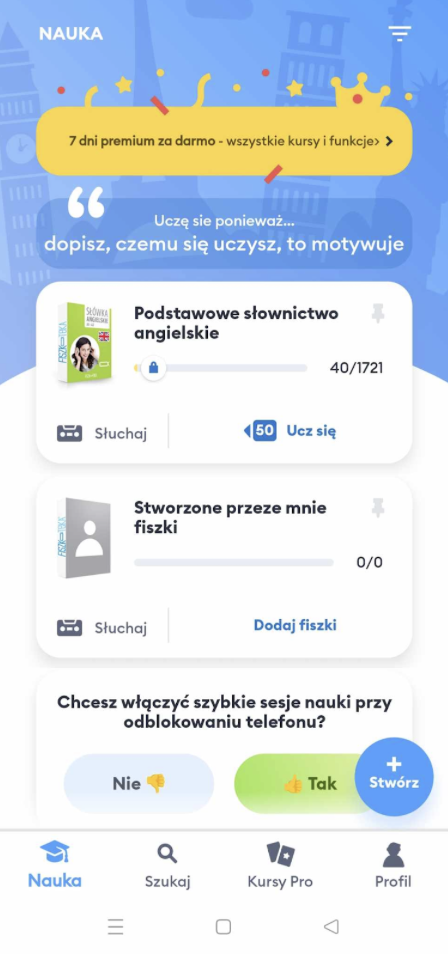
\includegraphics[width=0.3\textwidth]{chapters/chapter_3/fiszoteka.png}
    \caption{Aplikacja mobilna Fiszoteka.}
    \label{img:fiszoteka}
\end{figure}

Zalety:
\begin{itemize}[label=-]
    \item Dostępne talie językowe o różnych poziomach trudności
    \item Odczytanie przez lektora treści fiszki po zobaczeniu odpowiedzi
    \item Tryb słuchania, tytuł i treść fiszek są odczytywane po kolei przez lektora
    \item Dostęp do publicznych talii
    \item Można pobrać dokument PDF lub Mp3 z fiszek
\end{itemize}

Wady:
\begin{itemize}[label=-]
    \item Pełny dostęp do wszystkich funkcjonalności tylko za opłatą
    \item Dla bezpłatnej wersji ograniczenie liczby utworzonych fiszek do 300
    \item Reklamy w aplikacji
    \item Lektor w bezpłatnej wersji ograniczony do 20 dźwięków dziennie
    \item Brak trybu sterowania talii głosem
    \item Aplikacja ukierunkowana na uczenie się słówek
\end{itemize}

\subsection{Gizmo}

Aplikacja wykorzystuje narzędzia sztucznej inteligencji, które pozwalają na tworzenie zestawów fiszek na podstawie plików PDF, CSV lub filmów na platformie YouTube. Gizmo posiada zarówno stronę internetową, jak i aplikację mobilną na Androida i iOS.

\begin{figure}[H]
    \centering
    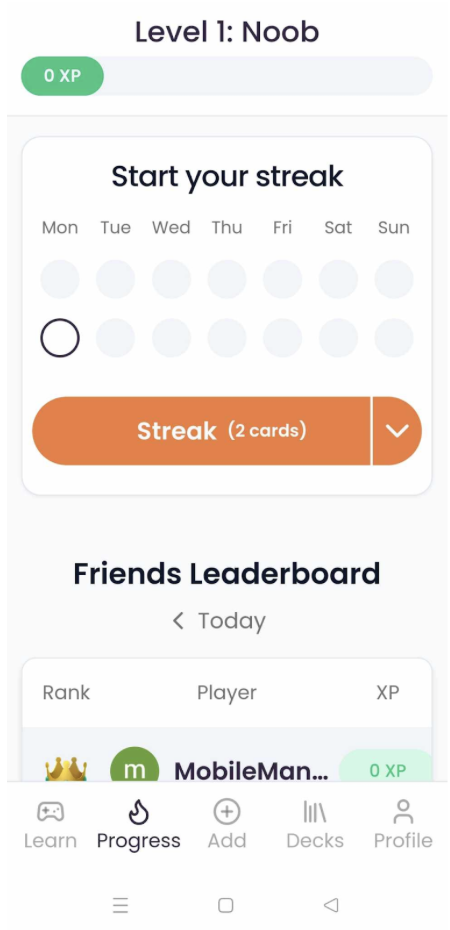
\includegraphics[width=0.3\textwidth]{chapters/chapter_3/gizmo.png}
    \caption{Aplikacja mobilna Gizmo.}
    \label{img:gizmo}
\end{figure}

Zalety:
\begin{itemize}[label=-]
    \item Brak reklam, brak opłat
    \item Zaawansowane zastosowanie AI do tworzenia fiszek
    \item Automatyczne tłumaczenie skanu na język angielski
    \item Szybki i prosty import fiszek z różnych źródeł
    \item Kalendarz passy (streak) zachęcający do nauki
    \item Przejrzysty interfejs
    \item Dostęp do publicznych talii
\end{itemize}

Wady:
\begin{itemize}[label=-]
    \item Nieumiejętne użycie AI przy tworzeniu, prowadzi do utworzenia bezsensownych talii
    \item Dużo niezagospodarowanej przestrzeni na ekranie w trybie uczenia
    \item Brak rankingu popularności talii użytkowników
    \item Domyślnie irytująca częstotliwość powiadomień
    \item Brak trybu sterowania talii głosem
\end{itemize}

\subsection{Flashcards}

Aplikacja dostępna tylko w wersji mobilnej. Ukierunkowana na uczenie się ze słuchu i tworzenie talii z użyciem mowy. Nieintuicyjny interfejs sprawia, że aplikacja jest nieprzyjazna dla nowych użytkowników.

\begin{figure}[H]
    \centering
    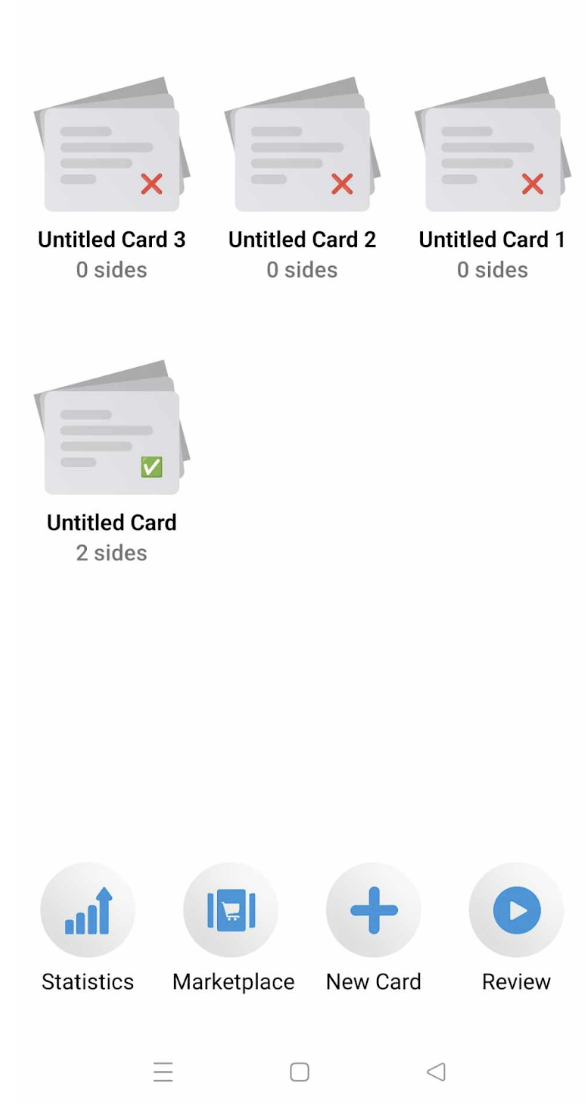
\includegraphics[width=0.3\textwidth]{chapters/chapter_3/flashcards.png}
    \caption{Aplikacja mobilna Flashcards.}
    \label{img:flashcards}
\end{figure}

Zalety:
\begin{itemize}[label=-]
    \item W trybie uczenia pozwala na korzystanie bez dotykania
    \item Możliwość tworzenia fiszek poprzez dyktowanie
    \item Brak reklam, brak opłat
\end{itemize}

Wady:
\begin{itemize}[label=-]
    \item Bardzo archaiczny interfejs
    \item Nieintuicyjny interfejs
    \item Skromna instrukcja korzystania
    \item W trybie uczenia można tylko słuchać i czekać na timer, nie ma nasłuchiwania haseł/komend
    \item Brak publicznych talii
\end{itemize}

\section{Analiza szans oraz zalet względem konkurencyjnych rozwiązań}

Podrozdział zawiera spis najważniejszych funkcjonalności, które odróżniają aplikację fiszki od innych produktów dostępnych na rynku.

\subsection{Szanse/Zalety względem konkurencyjnych rozwiązań}

Zalety:
\begin{itemize}[label=-]
    \item Sterowanie głosowe talii
    \item Generowanie treści fiszki, wykorzystując ChatGPT
    \item Ranking najpopularniejszych talii
\end{itemize}

\subsection{Wady względem konkurencyjnych rozwiązań}

Wady:
\begin{itemize}[label=-]
    \item Aplikacja dostępna tylko w języku angielskim uniemożliwia uczenie się języków obcych
    \item Brak narzędzi generowania zestawów talii z różnych formatów plików takich jak: CSV, mp4, PDF
    \item Brak możliwości generowania testów wielokrotnego wyboru lub prawda/fałsz
    \item Nie można eksportować talii do innych formatów plików takich jak PDF lub CSV
\end{itemize}

\section{Analiza ryzyka}

Podrozdział przedstawia analizę ryzyka, która ma na celu określenie i zrozumienie potencjalnych zagrożeń, które mogą wpłynąć na proces tworzenia projektu.


\newpage

\begin{longtable}{|p{2.3cm}|p{2.3cm}|p{2.3cm}|p{2.3cm}|p{2.3cm}|p{2.3cm}|}
    \hline
\textbf{Zidentyfiko- wane ryzyko [20]} & \textbf{Symptomy} & \textbf{Środki / Działania zapobiegawcze i szacowany poziom trudności ich wdrożenia} & \textbf{Środki / Działania minimalizujące wpływ na projekt – już po jego wystąpieniu i szacowany poziom trudności ich wdrożenia (1-10)} & \textbf{Ranga ryzyka (im niższa, tym mniejszy negatywny wpływ na projekt)} & \textbf{Prawdopodo- bieństwo wystąpienia (1-100\%)} \\
\hline
Błędy w kodzie [O] & Błędy w kompilacji, wyniki testów nie pokrywają się z oczekiwanym rezultatem  & Szybka identyfikacja błędów, wykonywanie testów oprogramowania & Poprawa kodu, testowanie na bieżąco nowo implementowanych funkcjonalności (4) & 10 & 80\% \\
\hline
Awaria sprzętu deweloperskiego [S] & Sprzęt przestaje działać, brak możliwości odzyskania danych & Częste commity na repozytorium & Działanie na ostatniej wersji z repozytorium (1) & 7 & 10\% \\
\hline
Niedobór umiejętności w zespole [L] & Problemy jednostek w poszczególnych zadaniach & Uzupełnianie wiedzy & Pomoc innych członków zespołu (2) & 7 & 70\% \\
\hline
Niezgodność czasowa zespołu [C]  & Osoba blokuje postęp nad projektem poprzez odpowiedzialność nad kluczowym elementem & Wcześniejsze zaplanowanie pracy & Wspólna praca nad kluczowym elementem zajęcie się zadaniami niepowiązanymi (5) & 6 & 80\% \\
\hline
Wybór nieodpowiedniej technologii [T] & Planowane rozwiązania nie są osiągalne przez wykorzystywane technologie & Dogłębna analiza potrzebnych technologii i ich możliwości/ograniczeń & Dopasowanie alternatywnych możliwych rozwiązań (8) & 5 & 50\% \\
\hline
Niedoszacowa- nie budżetu potrzebnego do utrzymania infrastruktury [B] & Budżet zbliża się do wyczerpania przed zaplanowanym terminem  & Analiza cenników wykorzystywanych produktów & Próba pozyskania inwestorów (10) & 10 & 80\% \\
\hline
ChatGPT 3.5 generuje bezsensowną treść dotycząca zagadnienia o którą został zapytany przez użytkownika [F] & Generowane treści nie nawiązują do zagadnienia, o które chat został zapytany & Próba sprecyzowania zapytania, które zostało przesłane do chatu w celu wygenerowania konkretniejszej treści & Użytkownik może zaakceptować lub odrzucić wygenerowaną treść. (4) & 7 & 50\% \\
\hline
    Przeglądarka niepoprawnie wczytuje stronę internetową [Ś] & Style strony nie wyglądają tak samo jak na stronie uruchomionej lokalnie lub na innych przeglądarkach. Pozycje elementów na stronie są inaczej rozmieszczone. & Próba dostosowania styli lub funkcjonalności do konkretnej przeglądarki.  & Uruchomienie strony internetowej na innej przeglądarce (3).   & 10 & 70\% \\
    \hline
\end{longtable}



    \chapter{Projekt w kontekście problemu}

\section{Omówienie zakresu projektu}

W odpowiedzi na zdefiniowany i omówiony w Rozdziale II problem, niniejszy projekt zakłada wytworzenie aplikacji edukacyjnej, która umożliwi naukę metodą wykorzystującą fiszki. Projekt obejmuje dostarczenie aplikacji webowej dostępnej z poziomu przeglądarki internetowej oraz aplikacji mobilnej dla urządzeń z systemem Android lub iOS. W zakres prac wlicza się także zbudowanie pełnej infrastruktury wspierającej aplikację - backend oraz serwer utrzymujący cały system.

\section{Proponowane rozwiązanie}

Projekt bazuje na kilku kluczowych założeniach, które mają na celu bezpośrednie rozwiązanie problemów opisanych w Rozdziale II:

\begin{itemize}
    \item obsługa głosowa: integracja obsługi głosowej aplikacji ma ułatwić korzystanie z niej w sytuacjach, w których użytkownik ma ograniczone możliwości fizycznej obsługi urządzenia. Dzięki temu nauka jest możliwa w każdych warunkach, co odpowiada na problem ograniczonej dostępności tradycyjnych metod nauki;
    \item narzędzie AI do tworzenia fiszek: udostępnienie narzędzia umożliwiającego automatyczne generowanie i dobieranie definicji/odpowiedzi do zagadnień w fiszkach. Pozwala przyśpieszyć i uprzystępnić proces redagowania fiszek.
\end{itemize}

\section{Grupa docelowa}

Główną grupę użytkowników stanowią uczniowie i studenci, a także osoby, które nie mają czasu na tradycyjną formę przyswajania wiedzy, na przykład czytanie lub naukę przy biurku w domowym zaciszu. Generowanie definicji przy użyciu programu ChatGPT pozwala na szybkie tworzenie zestawów fiszek, co może być bardzo wygodne dla osób ceniących sobie czas. Głosowa obsługa talii fiszek pozwala na wykonywanie sesji nauki w warunkach niesprzyjających innym formom uczenia się. Użytkownik ma możliwość powtórzenia materiału, wykonując inne obowiązki, takie jak gotowanie, sprzątanie lub inne czynności, którym nie trzeba poświęcać większej uwagi.

\section{Analiza rozwiązań konkurencji}

Ważnym aspektem tworzenia nowego produktu lub usługi jest analiza konkurencji. Dostrzeżenie wad i zalet konkurencyjnych rozwiązań pozwala na ulepszenie produktów dostępnych na rynku i dotarcie do nowej grupy klientów.

\subsection{Quizlet}

%\putimage{Aplikacja mobilna Quizlet.}{chapters/chapter_3/quizlet.png}{img:quizlet}{0.5\textwidth}

Jedna z pierwszych dostępnych na rynku aplikacja do fiszek. Utworzone w 2005 roku narzędzie do nauki zgromadziło ogromną bazę użytkowników szacowaną na około 50 milionów. Quizlet posiada stronę internetową i aplikacje mobilną dostępne na Android i IOS.

\begin{figure}[H]
    \centering
    
\includegraphics[width=0.3\textwidth]{chapters/chapter_3/quizlet.png}
    \caption{Aplikacja mobilna Quizlet.}
    \label{img:quizlet}
\end{figure}

Zalety:
\begin{itemize}[label=-]
    \item Możliwość tworzenia testów w różnych trybach: prawda/fałsz, wielokrotny wybór, pisemny
    \item Odczytanie przez lektora treści fiszki poprzez kliknięcie przycisku
    \item Dostęp do materiałów, które zostały zweryfikowane przez ekspertów
    \item Personalizacja fiszek za pomocą obrazów i dźwięków
    \item Pozwala na wyszukiwanie talii innych użytkowników
\end{itemize}

Wady:
\begin{itemize}[label=-]
    \item Reklamy w aplikacji
    \item Pełny dostęp do wszystkich funkcjonalności tylko za opłatą
    \item Brak rankingu popularności talii użytkowników, co pozwalałoby na łatwy dostęp do innych talii
    \item Brak trybu sterowania talii głosem
\end{itemize}

\subsection{Fiszkoteka}

Polski portal do nauki metodą fiszek ukierunkowany na naukę języków obcych. Oprócz strony internetowej aplikacja dostępna na system Android lub iOS.

\begin{figure}[H]
    \centering
    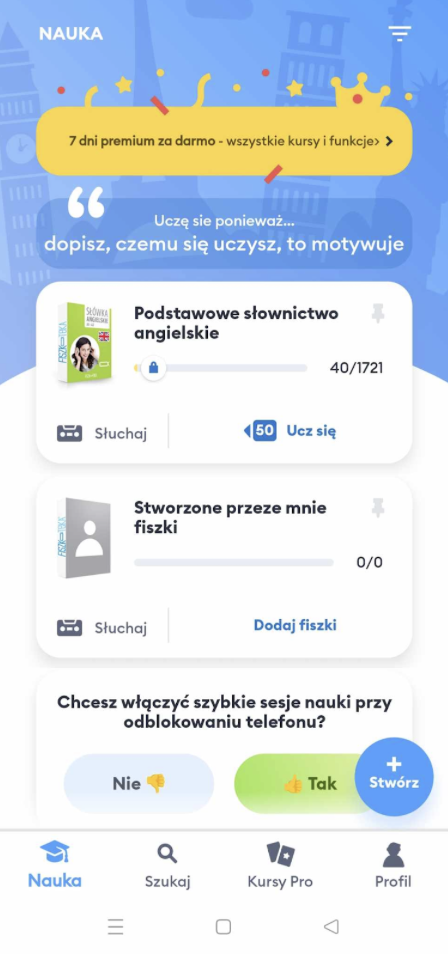
\includegraphics[width=0.3\textwidth]{chapters/chapter_3/fiszoteka.png}
    \caption{Aplikacja mobilna Fiszoteka.}
    \label{img:fiszoteka}
\end{figure}

Zalety:
\begin{itemize}[label=-]
    \item Dostępne talie językowe o różnych poziomach trudności
    \item Odczytanie przez lektora treści fiszki po zobaczeniu odpowiedzi
    \item Tryb słuchania, tytuł i treść fiszek są odczytywane po kolei przez lektora
    \item Dostęp do publicznych talii
    \item Można pobrać dokument PDF lub Mp3 z fiszek
\end{itemize}

Wady:
\begin{itemize}[label=-]
    \item Pełny dostęp do wszystkich funkcjonalności tylko za opłatą
    \item Dla bezpłatnej wersji ograniczenie liczby utworzonych fiszek do 300
    \item Reklamy w aplikacji
    \item Lektor w bezpłatnej wersji ograniczony do 20 dźwięków dziennie
    \item Brak trybu sterowania talii głosem
    \item Aplikacja ukierunkowana na uczenie się słówek
\end{itemize}

\subsection{Gizmo}

Aplikacja wykorzystuje narzędzia sztucznej inteligencji, które pozwalają na tworzenie zestawów fiszek na podstawie plików PDF, CSV lub filmów na platformie YouTube. Gizmo posiada zarówno stronę internetową, jak i aplikację mobilną na Androida i iOS.

\begin{figure}[H]
    \centering
    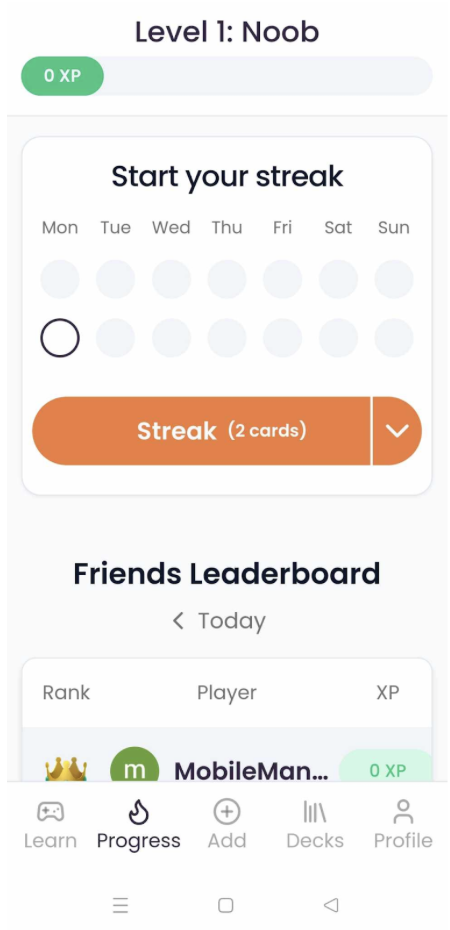
\includegraphics[width=0.3\textwidth]{chapters/chapter_3/gizmo.png}
    \caption{Aplikacja mobilna Gizmo.}
    \label{img:gizmo}
\end{figure}

Zalety:
\begin{itemize}[label=-]
    \item Brak reklam, brak opłat
    \item Zaawansowane zastosowanie AI do tworzenia fiszek
    \item Automatyczne tłumaczenie skanu na język angielski
    \item Szybki i prosty import fiszek z różnych źródeł
    \item Kalendarz passy (streak) zachęcający do nauki
    \item Przejrzysty interfejs
    \item Dostęp do publicznych talii
\end{itemize}

Wady:
\begin{itemize}[label=-]
    \item Nieumiejętne użycie AI przy tworzeniu, prowadzi do utworzenia bezsensownych talii
    \item Dużo niezagospodarowanej przestrzeni na ekranie w trybie uczenia
    \item Brak rankingu popularności talii użytkowników
    \item Domyślnie irytująca częstotliwość powiadomień
    \item Brak trybu sterowania talii głosem
\end{itemize}

\subsection{Flashcards}

Aplikacja dostępna tylko w wersji mobilnej. Ukierunkowana na uczenie się ze słuchu i tworzenie talii z użyciem mowy. Nieintuicyjny interfejs sprawia, że aplikacja jest nieprzyjazna dla nowych użytkowników.

\begin{figure}[H]
    \centering
    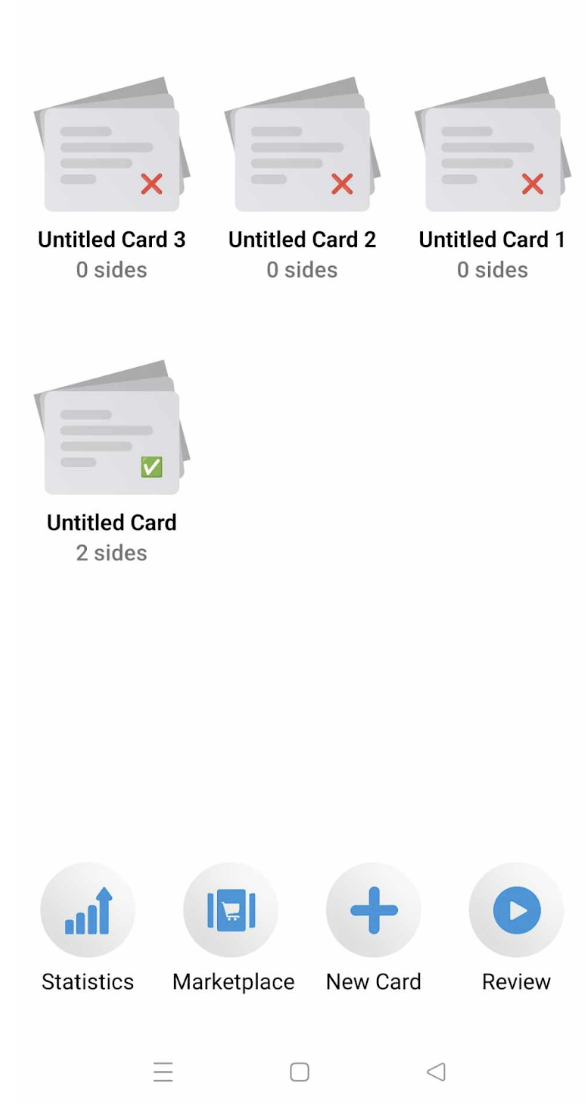
\includegraphics[width=0.3\textwidth]{chapters/chapter_3/flashcards.png}
    \caption{Aplikacja mobilna Flashcards.}
    \label{img:flashcards}
\end{figure}

Zalety:
\begin{itemize}[label=-]
    \item W trybie uczenia pozwala na korzystanie bez dotykania
    \item Możliwość tworzenia fiszek poprzez dyktowanie
    \item Brak reklam, brak opłat
\end{itemize}

Wady:
\begin{itemize}[label=-]
    \item Bardzo archaiczny interfejs
    \item Nieintuicyjny interfejs
    \item Skromna instrukcja korzystania
    \item W trybie uczenia można tylko słuchać i czekać na timer, nie ma nasłuchiwania haseł/komend
    \item Brak publicznych talii
\end{itemize}

\section{Analiza szans oraz zalet względem konkurencyjnych rozwiązań}

Podrozdział zawiera spis najważniejszych funkcjonalności, które odróżniają aplikację fiszki od innych produktów dostępnych na rynku.

\subsection{Szanse/Zalety względem konkurencyjnych rozwiązań}

Zalety:
\begin{itemize}[label=-]
    \item Sterowanie głosowe talii
    \item Generowanie treści fiszki, wykorzystując ChatGPT
    \item Ranking najpopularniejszych talii
\end{itemize}

\subsection{Wady względem konkurencyjnych rozwiązań}

Wady:
\begin{itemize}[label=-]
    \item Aplikacja dostępna tylko w języku angielskim uniemożliwia uczenie się języków obcych
    \item Brak narzędzi generowania zestawów talii z różnych formatów plików takich jak: CSV, mp4, PDF
    \item Brak możliwości generowania testów wielokrotnego wyboru lub prawda/fałsz
    \item Nie można eksportować talii do innych formatów plików takich jak PDF lub CSV
\end{itemize}

\section{Analiza ryzyka}

Podrozdział przedstawia analizę ryzyka, która ma na celu określenie i zrozumienie potencjalnych zagrożeń, które mogą wpłynąć na proces tworzenia projektu.


\newpage

\begin{longtable}{|p{2.3cm}|p{2.3cm}|p{2.3cm}|p{2.3cm}|p{2.3cm}|p{2.3cm}|}
    \hline
\textbf{Zidentyfiko- wane ryzyko [20]} & \textbf{Symptomy} & \textbf{Środki / Działania zapobiegawcze i szacowany poziom trudności ich wdrożenia} & \textbf{Środki / Działania minimalizujące wpływ na projekt – już po jego wystąpieniu i szacowany poziom trudności ich wdrożenia (1-10)} & \textbf{Ranga ryzyka (im niższa, tym mniejszy negatywny wpływ na projekt)} & \textbf{Prawdopodo- bieństwo wystąpienia (1-100\%)} \\
\hline
Błędy w kodzie [O] & Błędy w kompilacji, wyniki testów nie pokrywają się z oczekiwanym rezultatem  & Szybka identyfikacja błędów, wykonywanie testów oprogramowania & Poprawa kodu, testowanie na bieżąco nowo implementowanych funkcjonalności (4) & 10 & 80\% \\
\hline
Awaria sprzętu deweloperskiego [S] & Sprzęt przestaje działać, brak możliwości odzyskania danych & Częste commity na repozytorium & Działanie na ostatniej wersji z repozytorium (1) & 7 & 10\% \\
\hline
Niedobór umiejętności w zespole [L] & Problemy jednostek w poszczególnych zadaniach & Uzupełnianie wiedzy & Pomoc innych członków zespołu (2) & 7 & 70\% \\
\hline
Niezgodność czasowa zespołu [C]  & Osoba blokuje postęp nad projektem poprzez odpowiedzialność nad kluczowym elementem & Wcześniejsze zaplanowanie pracy & Wspólna praca nad kluczowym elementem zajęcie się zadaniami niepowiązanymi (5) & 6 & 80\% \\
\hline
Wybór nieodpowiedniej technologii [T] & Planowane rozwiązania nie są osiągalne przez wykorzystywane technologie & Dogłębna analiza potrzebnych technologii i ich możliwości/ograniczeń & Dopasowanie alternatywnych możliwych rozwiązań (8) & 5 & 50\% \\
\hline
Niedoszacowa- nie budżetu potrzebnego do utrzymania infrastruktury [B] & Budżet zbliża się do wyczerpania przed zaplanowanym terminem  & Analiza cenników wykorzystywanych produktów & Próba pozyskania inwestorów (10) & 10 & 80\% \\
\hline
ChatGPT 3.5 generuje bezsensowną treść dotycząca zagadnienia o którą został zapytany przez użytkownika [F] & Generowane treści nie nawiązują do zagadnienia, o które chat został zapytany & Próba sprecyzowania zapytania, które zostało przesłane do chatu w celu wygenerowania konkretniejszej treści & Użytkownik może zaakceptować lub odrzucić wygenerowaną treść. (4) & 7 & 50\% \\
\hline
    Przeglądarka niepoprawnie wczytuje stronę internetową [Ś] & Style strony nie wyglądają tak samo jak na stronie uruchomionej lokalnie lub na innych przeglądarkach. Pozycje elementów na stronie są inaczej rozmieszczone. & Próba dostosowania styli lub funkcjonalności do konkretnej przeglądarki.  & Uruchomienie strony internetowej na innej przeglądarce (3).   & 10 & 70\% \\
    \hline
\end{longtable}



    \chapter{Projekt w kontekście problemu}

\section{Omówienie zakresu projektu}

W odpowiedzi na zdefiniowany i omówiony w Rozdziale II problem, niniejszy projekt zakłada wytworzenie aplikacji edukacyjnej, która umożliwi naukę metodą wykorzystującą fiszki. Projekt obejmuje dostarczenie aplikacji webowej dostępnej z poziomu przeglądarki internetowej oraz aplikacji mobilnej dla urządzeń z systemem Android lub iOS. W zakres prac wlicza się także zbudowanie pełnej infrastruktury wspierającej aplikację - backend oraz serwer utrzymujący cały system.

\section{Proponowane rozwiązanie}

Projekt bazuje na kilku kluczowych założeniach, które mają na celu bezpośrednie rozwiązanie problemów opisanych w Rozdziale II:

\begin{itemize}
    \item obsługa głosowa: integracja obsługi głosowej aplikacji ma ułatwić korzystanie z niej w sytuacjach, w których użytkownik ma ograniczone możliwości fizycznej obsługi urządzenia. Dzięki temu nauka jest możliwa w każdych warunkach, co odpowiada na problem ograniczonej dostępności tradycyjnych metod nauki;
    \item narzędzie AI do tworzenia fiszek: udostępnienie narzędzia umożliwiającego automatyczne generowanie i dobieranie definicji/odpowiedzi do zagadnień w fiszkach. Pozwala przyśpieszyć i uprzystępnić proces redagowania fiszek.
\end{itemize}

\section{Grupa docelowa}

Główną grupę użytkowników stanowią uczniowie i studenci, a także osoby, które nie mają czasu na tradycyjną formę przyswajania wiedzy, na przykład czytanie lub naukę przy biurku w domowym zaciszu. Generowanie definicji przy użyciu programu ChatGPT pozwala na szybkie tworzenie zestawów fiszek, co może być bardzo wygodne dla osób ceniących sobie czas. Głosowa obsługa talii fiszek pozwala na wykonywanie sesji nauki w warunkach niesprzyjających innym formom uczenia się. Użytkownik ma możliwość powtórzenia materiału, wykonując inne obowiązki, takie jak gotowanie, sprzątanie lub inne czynności, którym nie trzeba poświęcać większej uwagi.

\section{Analiza rozwiązań konkurencji}

Ważnym aspektem tworzenia nowego produktu lub usługi jest analiza konkurencji. Dostrzeżenie wad i zalet konkurencyjnych rozwiązań pozwala na ulepszenie produktów dostępnych na rynku i dotarcie do nowej grupy klientów.

\subsection{Quizlet}

%\putimage{Aplikacja mobilna Quizlet.}{chapters/chapter_3/quizlet.png}{img:quizlet}{0.5\textwidth}

Jedna z pierwszych dostępnych na rynku aplikacja do fiszek. Utworzone w 2005 roku narzędzie do nauki zgromadziło ogromną bazę użytkowników szacowaną na około 50 milionów. Quizlet posiada stronę internetową i aplikacje mobilną dostępne na Android i IOS.

\begin{figure}[H]
    \centering
    
\includegraphics[width=0.3\textwidth]{chapters/chapter_3/quizlet.png}
    \caption{Aplikacja mobilna Quizlet.}
    \label{img:quizlet}
\end{figure}

Zalety:
\begin{itemize}[label=-]
    \item Możliwość tworzenia testów w różnych trybach: prawda/fałsz, wielokrotny wybór, pisemny
    \item Odczytanie przez lektora treści fiszki poprzez kliknięcie przycisku
    \item Dostęp do materiałów, które zostały zweryfikowane przez ekspertów
    \item Personalizacja fiszek za pomocą obrazów i dźwięków
    \item Pozwala na wyszukiwanie talii innych użytkowników
\end{itemize}

Wady:
\begin{itemize}[label=-]
    \item Reklamy w aplikacji
    \item Pełny dostęp do wszystkich funkcjonalności tylko za opłatą
    \item Brak rankingu popularności talii użytkowników, co pozwalałoby na łatwy dostęp do innych talii
    \item Brak trybu sterowania talii głosem
\end{itemize}

\subsection{Fiszkoteka}

Polski portal do nauki metodą fiszek ukierunkowany na naukę języków obcych. Oprócz strony internetowej aplikacja dostępna na system Android lub iOS.

\begin{figure}[H]
    \centering
    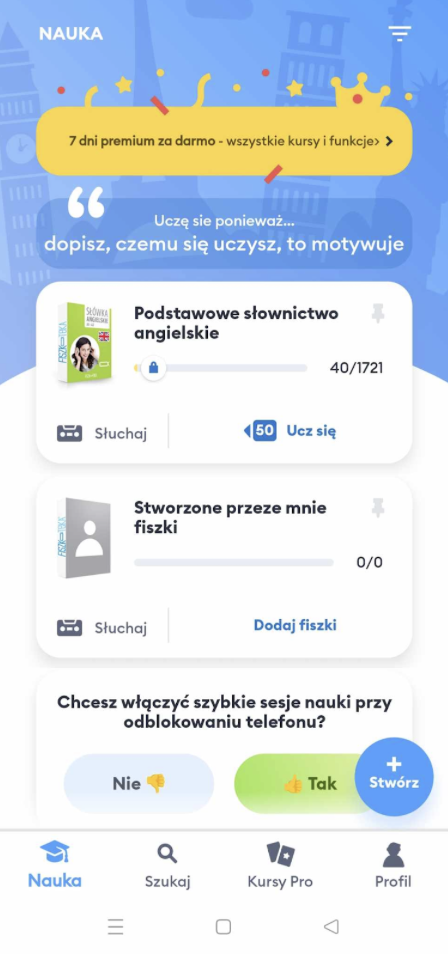
\includegraphics[width=0.3\textwidth]{chapters/chapter_3/fiszoteka.png}
    \caption{Aplikacja mobilna Fiszoteka.}
    \label{img:fiszoteka}
\end{figure}

Zalety:
\begin{itemize}[label=-]
    \item Dostępne talie językowe o różnych poziomach trudności
    \item Odczytanie przez lektora treści fiszki po zobaczeniu odpowiedzi
    \item Tryb słuchania, tytuł i treść fiszek są odczytywane po kolei przez lektora
    \item Dostęp do publicznych talii
    \item Można pobrać dokument PDF lub Mp3 z fiszek
\end{itemize}

Wady:
\begin{itemize}[label=-]
    \item Pełny dostęp do wszystkich funkcjonalności tylko za opłatą
    \item Dla bezpłatnej wersji ograniczenie liczby utworzonych fiszek do 300
    \item Reklamy w aplikacji
    \item Lektor w bezpłatnej wersji ograniczony do 20 dźwięków dziennie
    \item Brak trybu sterowania talii głosem
    \item Aplikacja ukierunkowana na uczenie się słówek
\end{itemize}

\subsection{Gizmo}

Aplikacja wykorzystuje narzędzia sztucznej inteligencji, które pozwalają na tworzenie zestawów fiszek na podstawie plików PDF, CSV lub filmów na platformie YouTube. Gizmo posiada zarówno stronę internetową, jak i aplikację mobilną na Androida i iOS.

\begin{figure}[H]
    \centering
    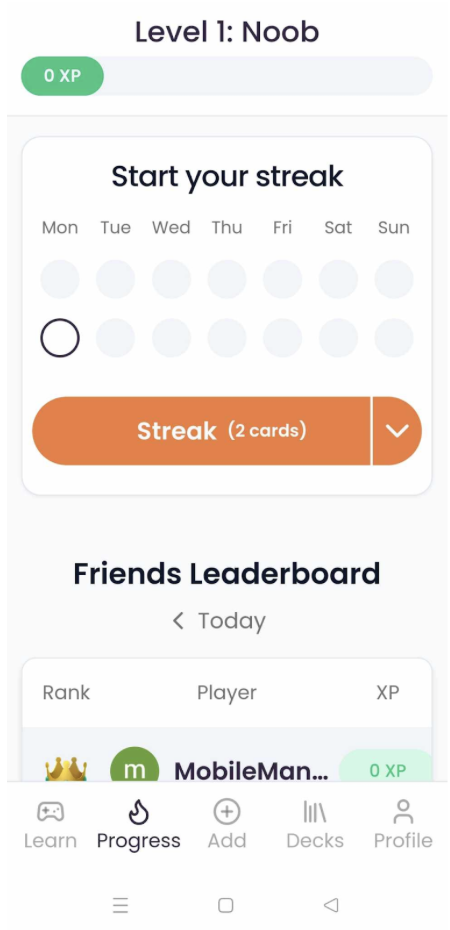
\includegraphics[width=0.3\textwidth]{chapters/chapter_3/gizmo.png}
    \caption{Aplikacja mobilna Gizmo.}
    \label{img:gizmo}
\end{figure}

Zalety:
\begin{itemize}[label=-]
    \item Brak reklam, brak opłat
    \item Zaawansowane zastosowanie AI do tworzenia fiszek
    \item Automatyczne tłumaczenie skanu na język angielski
    \item Szybki i prosty import fiszek z różnych źródeł
    \item Kalendarz passy (streak) zachęcający do nauki
    \item Przejrzysty interfejs
    \item Dostęp do publicznych talii
\end{itemize}

Wady:
\begin{itemize}[label=-]
    \item Nieumiejętne użycie AI przy tworzeniu, prowadzi do utworzenia bezsensownych talii
    \item Dużo niezagospodarowanej przestrzeni na ekranie w trybie uczenia
    \item Brak rankingu popularności talii użytkowników
    \item Domyślnie irytująca częstotliwość powiadomień
    \item Brak trybu sterowania talii głosem
\end{itemize}

\subsection{Flashcards}

Aplikacja dostępna tylko w wersji mobilnej. Ukierunkowana na uczenie się ze słuchu i tworzenie talii z użyciem mowy. Nieintuicyjny interfejs sprawia, że aplikacja jest nieprzyjazna dla nowych użytkowników.

\begin{figure}[H]
    \centering
    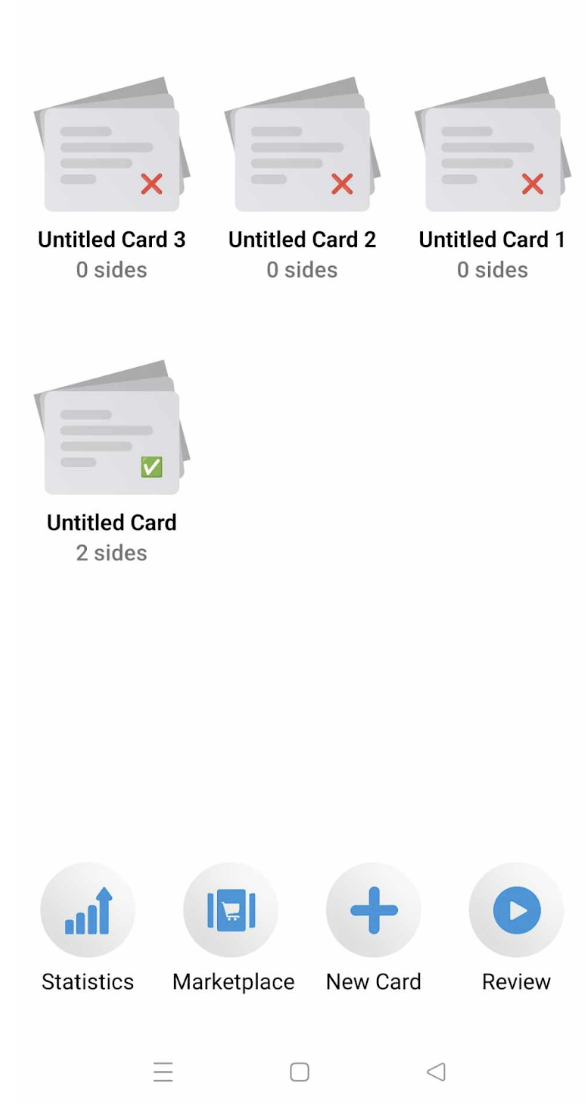
\includegraphics[width=0.3\textwidth]{chapters/chapter_3/flashcards.png}
    \caption{Aplikacja mobilna Flashcards.}
    \label{img:flashcards}
\end{figure}

Zalety:
\begin{itemize}[label=-]
    \item W trybie uczenia pozwala na korzystanie bez dotykania
    \item Możliwość tworzenia fiszek poprzez dyktowanie
    \item Brak reklam, brak opłat
\end{itemize}

Wady:
\begin{itemize}[label=-]
    \item Bardzo archaiczny interfejs
    \item Nieintuicyjny interfejs
    \item Skromna instrukcja korzystania
    \item W trybie uczenia można tylko słuchać i czekać na timer, nie ma nasłuchiwania haseł/komend
    \item Brak publicznych talii
\end{itemize}

\section{Analiza szans oraz zalet względem konkurencyjnych rozwiązań}

Podrozdział zawiera spis najważniejszych funkcjonalności, które odróżniają aplikację fiszki od innych produktów dostępnych na rynku.

\subsection{Szanse/Zalety względem konkurencyjnych rozwiązań}

Zalety:
\begin{itemize}[label=-]
    \item Sterowanie głosowe talii
    \item Generowanie treści fiszki, wykorzystując ChatGPT
    \item Ranking najpopularniejszych talii
\end{itemize}

\subsection{Wady względem konkurencyjnych rozwiązań}

Wady:
\begin{itemize}[label=-]
    \item Aplikacja dostępna tylko w języku angielskim uniemożliwia uczenie się języków obcych
    \item Brak narzędzi generowania zestawów talii z różnych formatów plików takich jak: CSV, mp4, PDF
    \item Brak możliwości generowania testów wielokrotnego wyboru lub prawda/fałsz
    \item Nie można eksportować talii do innych formatów plików takich jak PDF lub CSV
\end{itemize}

\section{Analiza ryzyka}

Podrozdział przedstawia analizę ryzyka, która ma na celu określenie i zrozumienie potencjalnych zagrożeń, które mogą wpłynąć na proces tworzenia projektu.


\newpage

\begin{longtable}{|p{2.3cm}|p{2.3cm}|p{2.3cm}|p{2.3cm}|p{2.3cm}|p{2.3cm}|}
    \hline
\textbf{Zidentyfiko- wane ryzyko [20]} & \textbf{Symptomy} & \textbf{Środki / Działania zapobiegawcze i szacowany poziom trudności ich wdrożenia} & \textbf{Środki / Działania minimalizujące wpływ na projekt – już po jego wystąpieniu i szacowany poziom trudności ich wdrożenia (1-10)} & \textbf{Ranga ryzyka (im niższa, tym mniejszy negatywny wpływ na projekt)} & \textbf{Prawdopodo- bieństwo wystąpienia (1-100\%)} \\
\hline
Błędy w kodzie [O] & Błędy w kompilacji, wyniki testów nie pokrywają się z oczekiwanym rezultatem  & Szybka identyfikacja błędów, wykonywanie testów oprogramowania & Poprawa kodu, testowanie na bieżąco nowo implementowanych funkcjonalności (4) & 10 & 80\% \\
\hline
Awaria sprzętu deweloperskiego [S] & Sprzęt przestaje działać, brak możliwości odzyskania danych & Częste commity na repozytorium & Działanie na ostatniej wersji z repozytorium (1) & 7 & 10\% \\
\hline
Niedobór umiejętności w zespole [L] & Problemy jednostek w poszczególnych zadaniach & Uzupełnianie wiedzy & Pomoc innych członków zespołu (2) & 7 & 70\% \\
\hline
Niezgodność czasowa zespołu [C]  & Osoba blokuje postęp nad projektem poprzez odpowiedzialność nad kluczowym elementem & Wcześniejsze zaplanowanie pracy & Wspólna praca nad kluczowym elementem zajęcie się zadaniami niepowiązanymi (5) & 6 & 80\% \\
\hline
Wybór nieodpowiedniej technologii [T] & Planowane rozwiązania nie są osiągalne przez wykorzystywane technologie & Dogłębna analiza potrzebnych technologii i ich możliwości/ograniczeń & Dopasowanie alternatywnych możliwych rozwiązań (8) & 5 & 50\% \\
\hline
Niedoszacowa- nie budżetu potrzebnego do utrzymania infrastruktury [B] & Budżet zbliża się do wyczerpania przed zaplanowanym terminem  & Analiza cenników wykorzystywanych produktów & Próba pozyskania inwestorów (10) & 10 & 80\% \\
\hline
ChatGPT 3.5 generuje bezsensowną treść dotycząca zagadnienia o którą został zapytany przez użytkownika [F] & Generowane treści nie nawiązują do zagadnienia, o które chat został zapytany & Próba sprecyzowania zapytania, które zostało przesłane do chatu w celu wygenerowania konkretniejszej treści & Użytkownik może zaakceptować lub odrzucić wygenerowaną treść. (4) & 7 & 50\% \\
\hline
    Przeglądarka niepoprawnie wczytuje stronę internetową [Ś] & Style strony nie wyglądają tak samo jak na stronie uruchomionej lokalnie lub na innych przeglądarkach. Pozycje elementów na stronie są inaczej rozmieszczone. & Próba dostosowania styli lub funkcjonalności do konkretnej przeglądarki.  & Uruchomienie strony internetowej na innej przeglądarce (3).   & 10 & 70\% \\
    \hline
\end{longtable}



    \printbibliography[title={Bibliografia}]
%    \printbibliography[title={Bibliografia}, heading=bibintoc]

\end{document}
